%             
% Hall D Note
% 
\documentclass[12pt]{article}


\usepackage{color}

% ===    Set a true/false value for PDF hyper marks  

\newif\ifhyprf
%\hyprffalse   
\hyprftrue

\RequirePackage{ifpdf}
  
\ifpdf
    \pdfoutput=1        % we are running PDFLaTeX
    \pdftrue
\else
    \pdffalse           % we are not running PDFLaTeX
\fi

\ifpdf
  \pdfcompresslevel=9
  \usepackage[pdftex]{graphicx}
%  \usepackage{thumbpdf}
  \definecolor{rltred}{rgb}{0.75,0,0}
  \definecolor{rltgreen}{rgb}{0,0.3,0}
  \definecolor{rltblue}{rgb}{0,0,0.75}
  \definecolor{rltdarkgreen}{rgb}{0.1,0.6,0.1}
  \ifhyprf
     \usepackage[pdftex,
         colorlinks=true,
         urlcolor=rltblue,       % \href{...}{...} external (URL)
         filecolor=rltgreen,     % \href{...} local file
         linkcolor=rltred,       % \ref{...} and \pageref{...}
         citecolor=rltdarkgreen, % citations
         pagebackref,
         pdfpagemode=None,
         pdftitle={Civil Reference Concepts for BDX},
         pdfauthor={many},
         pdfsubject={Civil Reference Concepts for BDX},
         pdfkeywords={JLab Beam Dump Experiment}]{hyperref}
  \fi
  \usepackage{pdfcolmk}
  \DeclareGraphicsExtensions{.pdf,.png,.jpg}
\else
  \usepackage{graphicx}
  \DeclareGraphicsExtensions{.eps,.epsi,.ps,.eps.gz,.epsi.gz,.ps.gz}
\fi

\setlength{\textwidth}{6.0in}
%\setlength{\textheight}{9.5in}
\setlength{\textheight}{8.75in}
\setlength{\evensidemargin}{0.25in}
\setlength{\oddsidemargin}{0.25in}
\setlength{\topmargin}{-0.25in}
\setlength{\footskip}{0.25in}
%\setlength{\parindent}{0pt}
%\setlength{\parskip}{0in}
\usepackage{graphicx,lscape,rotating}
\pagenumbering{arabic}
%\input epsf
\usepackage[utf8]{inputenc}

\begin{document}

\begin{flushright}
GlueX-doc-5373\\
github: eltonssmith/reports/MWPC\_production\_testing\\
***DRAFT*** November 24, 2021
\end{flushright}



%\pagestyle{myheadings}
%\markright{BDX-NOTE-2015-002}

%%%%%%%%%%%%%%%%%%%%%%%%%%%%%%%%%  TITLE %%%%%%%%%%%%%%%%%%%%%%%%%%%%%%%%
\begin{center}
{\Large \bf Production Testing of MWPCs for CPP}\\*[0.5cm]
\end{center}
%%%%%%%%%%%%%%%%%%%%%%%%%%%%%%%  AUTHORS %%%%%%%%%%%%%%%%%%%%%%%%%%%%%%%% 

\begin{center}   
{\sc  E.S. Smith, R. Miskimen, I. Larin, B. Zilhmann and A. Austregesilo}\\  
\end{center}

%\tableofcontents

\section{Introduction}
We are preparing the multi-wire proportional chambers (MWPCs) for the CPP\cite{CPPexp} and NPP\cite{NPPexp}. The MWPCs were designed and built at the University of Massachusetts, Amherst, by Rory Miskimen and his students. A detailed report on the design, construction, performance and acceptance testing is available in Ref. \cite{hdnote5080}. Eight chambers were built and delivered to Jefferson Lab. Six are required for the experiment, which leaves two spares. They are currently being tested systematically with cosmic rays in EEL 126. Each is identified by a unique name taken from the ``Lord of the Rings" trilogy by J.R.R. Tolkien: Arwen, Bilbo, Celeborn, Denethor, Ewoyen, Foldo, Galadriel and Haldor. This report summarizes the results of the production tests with cosmic rays at JLab.

\section{Requirements}
The MWPCs are used to reject muon pairs that might contaminate our sample of pion pairs. The proposal specifies that we need to limit the fraction of muons in the signal to $<$0.1\% and there are approximately ten times more muon pairs than pion pairs in the threshold region. Therefore, we require that our misidentification of two muons be less than $10^{-4}$, or less than $10^{-2}$ per muon. We estimate the efficiency required per MWPC plane to achieve this goal in two ways: 1) compute the probability of missing a muon track when it traverses six planes as a function of the per plane efficiency, and 2) using only the last two planes to tag two (muon) tracks, which are not reachable by hadrons. In the first instance we require that the per track inefficiency be less than 0.01, while in the second instance we require that missing two tracks be less than 0.0001. Assuming binomial probabilities of missing hits, we plot the track or two-track inefficiencies as a function of the per plane efficiency in Fig.\,\ref{fig:Ineff_muons}. Both estimates show that our goals can be achieved with a per plane efficiency of $>$ 97\%.

\begin{figure}[tbph]
\begin{center}
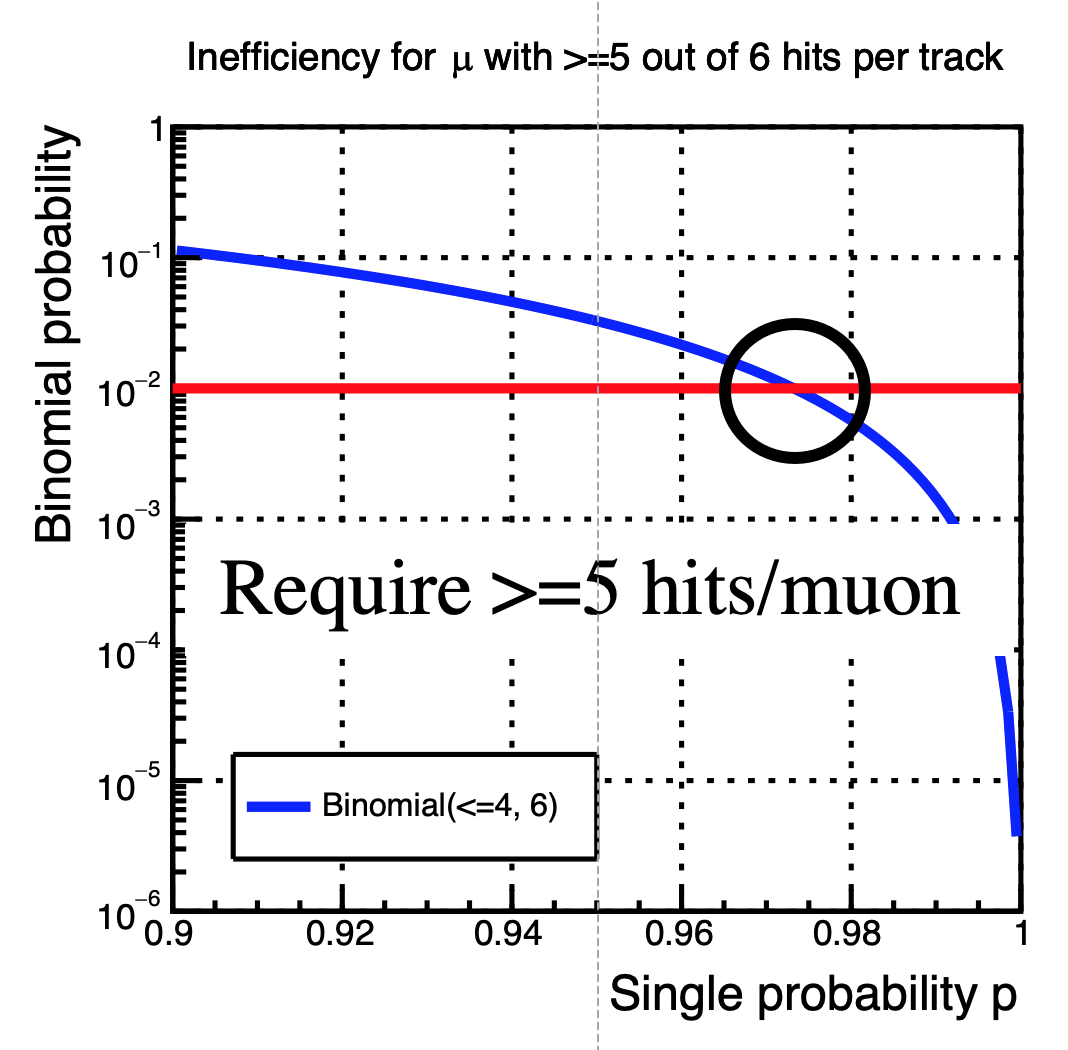
\includegraphics[height=6cm,clip=true]{Ineff_track}
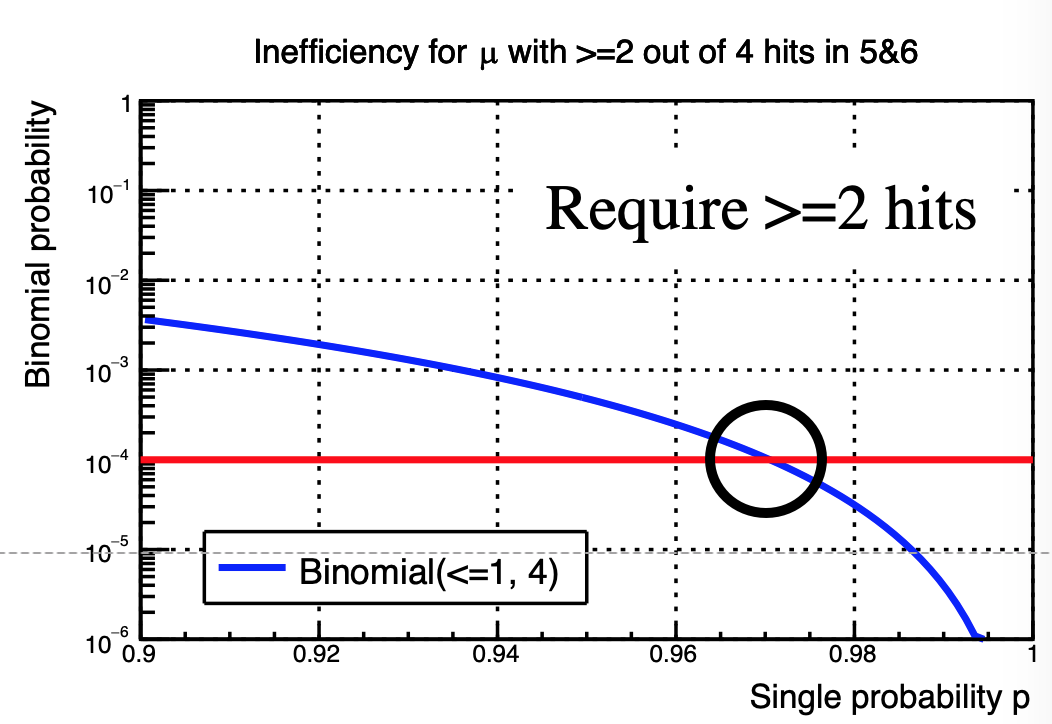
\includegraphics[height=6cm,clip=true]{Ineff_5-6}
\caption{Left) Probability to miss a track as a function of the per plane efficiency. Right) Probability to miss two muon tracks passing through planes 5 and 6 at the end of the muon stack. 
\label{fig:Ineff_muons}}
\end{center}
\end{figure} 

\section{Setup}
The experimental setup consists of a single MWPC sandwiched between two scintillators, as shown in Figs.\,\ref{fig:EEL126_test_elevation} and \ref{fig:EEL126_test_plan}.
Each scintillator is $1.27\times20\times120$ cm$^3$ and is positioned perpendicular to the orientation of wires in the MWPC. The scintillators are used for triggering
on cosmic rays and cover a 20-cm length of most of the wires in the chamber. The trigger requires pulses above threshold on two pmts in the top scintillator and one pmt in the bottom scintillator. The trigger rate is about 22\,Hz and constant throughout the testing of all MWPCs. The scintillators are read out with four channels of a JLab 250\,MHz Flash ADC and cosmic-ray tracks can be selected cleanly without reference to information from the MWPCs.\footnote{The Flash 250 MHz used to readout the scintillators had some stuck bits that needed to be ignored in software, but this did not affect our ability to select clean triggering tracks.} The MWPCs were readout by two JLab 125\,MHz Flash ADCs (144 wires). Full waveforms were recorded for all FADCs, 100 samples (400 ns) for the FADC-250 and 300 samples (2.4 $\mu$s) from the two FADC-125s. As an example, we show the MWPC waveforms for the first 10 events in R184 (Denethor) in Fig.\,\ref{fig:Waveform_Denethor_R184}. The printed parameters do not have the pedestal subtracted; the nominal pedestal is 100 counts and there are 300 samples.

The energies deposited in both the scintillators and the MWPCs are estimated using the integral of the waveform above pedestal. The times of the pulses are taken from the emulation of the hardware, which estimates the leading edge from the first samples above threshold. For the scintillators, the resolution of the time measurement is dominated by the sampling time of 4\,ns that produce artificial peaks in the time and position distributions. 

Each MWPC was placed on the test table, one at a time, and positioned in the same relative position relative to the scintillators. The detectors were aligned by hand but reproducibility was probably at the level of one cm. Gas was connected to the chamber and flushed for about 24 hours. The MWPC was then brought up to the operating  voltage of 1765\,V, which corresponds to the nominal gain of 10$^5$.  The voltage was ramped up slowly checking the current draw. All MWPCs draw about 3-5 $\mu$A at the nominal voltage. Considering the read back reproducibility of about 2 $\mu$A, the current draw is unchanged up to a voltage of about 1900 V 
(Fig.\,\ref{fig:Current_draw_Frodo}). Data were taken for several hours, usually overnight, before the next MWPC was replaced in the test setup. The present study only uses the beginning of each run.

      
\begin{figure}[tbph]
\begin{center}
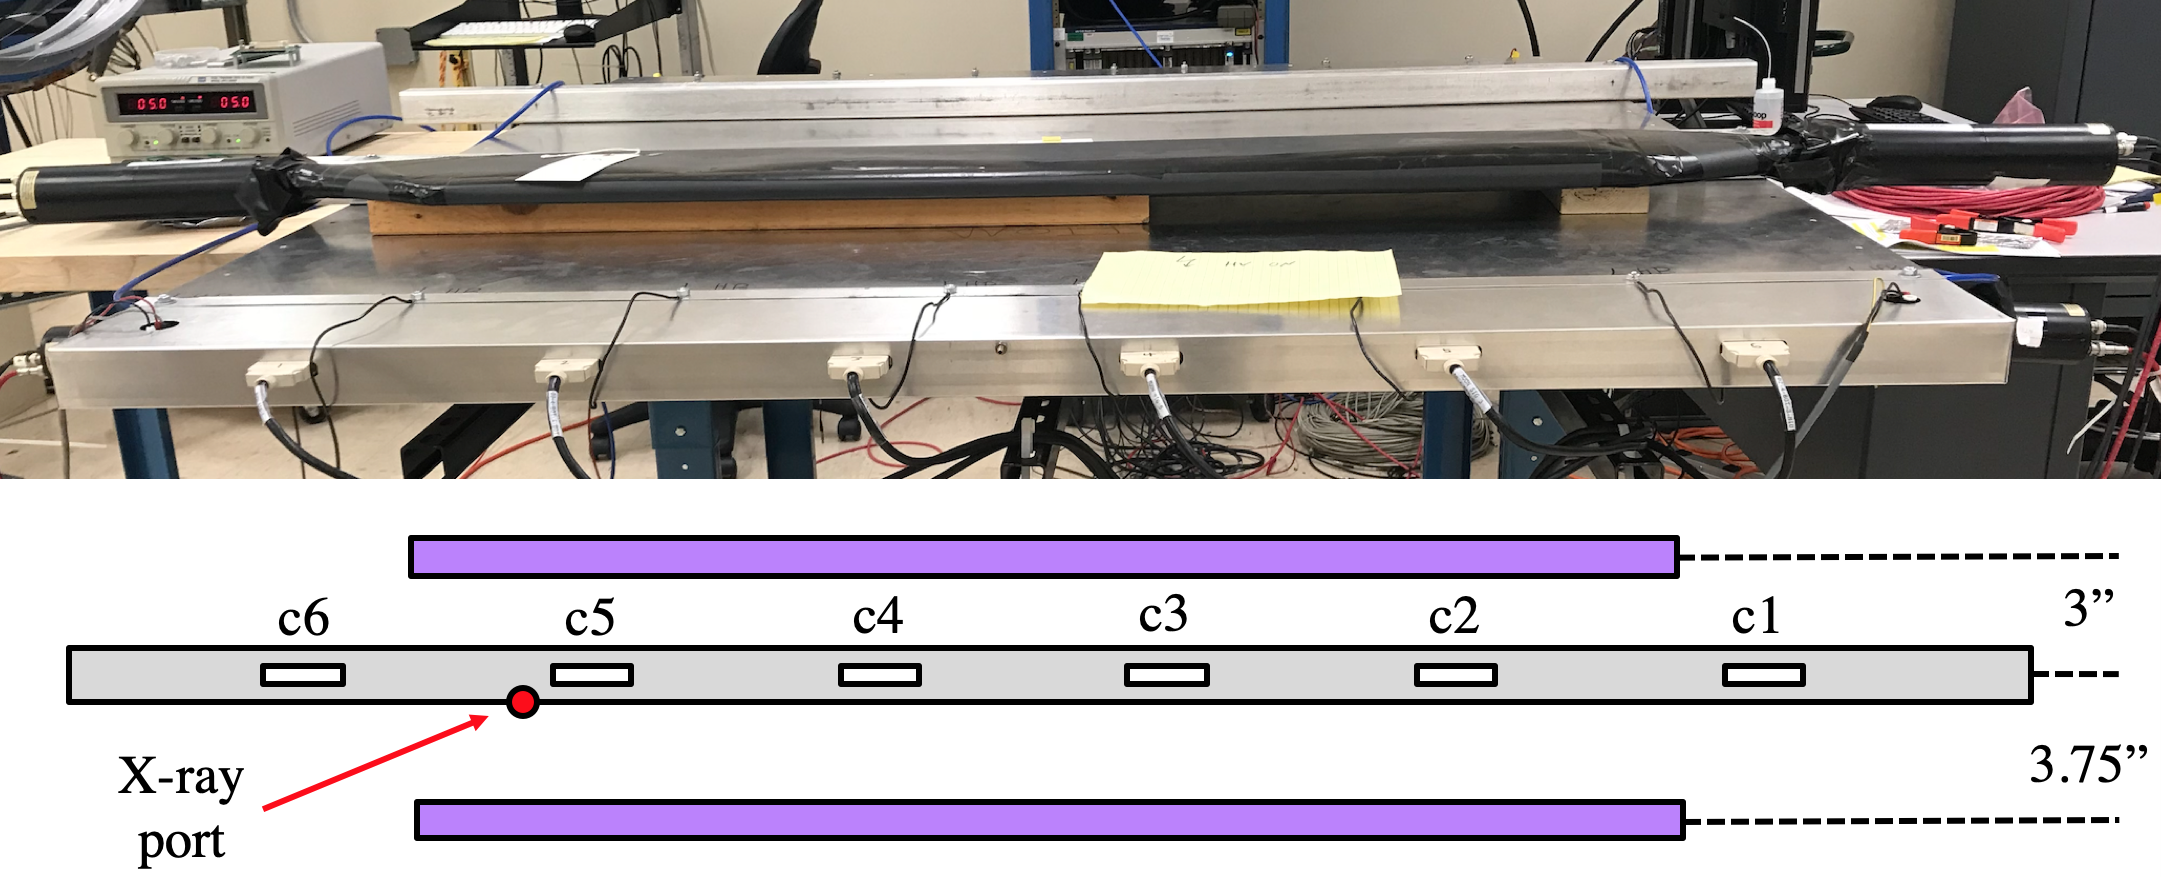
\includegraphics[height=6cm,clip=true]{EEL126_test_elevation}
\caption{Side view of cosmic-ray test setup in EEL126. Top) Photo of setup; the top scintillator paddle and MWPC connectors are visible. Bottom) Schematic of setup, showing
the distances between scintillators and MWPC as well as the approximate dimensions of the active scintillator relative to the MWPC plane.
\label{fig:EEL126_test_elevation}}
\end{center}
\end{figure}     


\begin{figure}[tbph]
\begin{center}
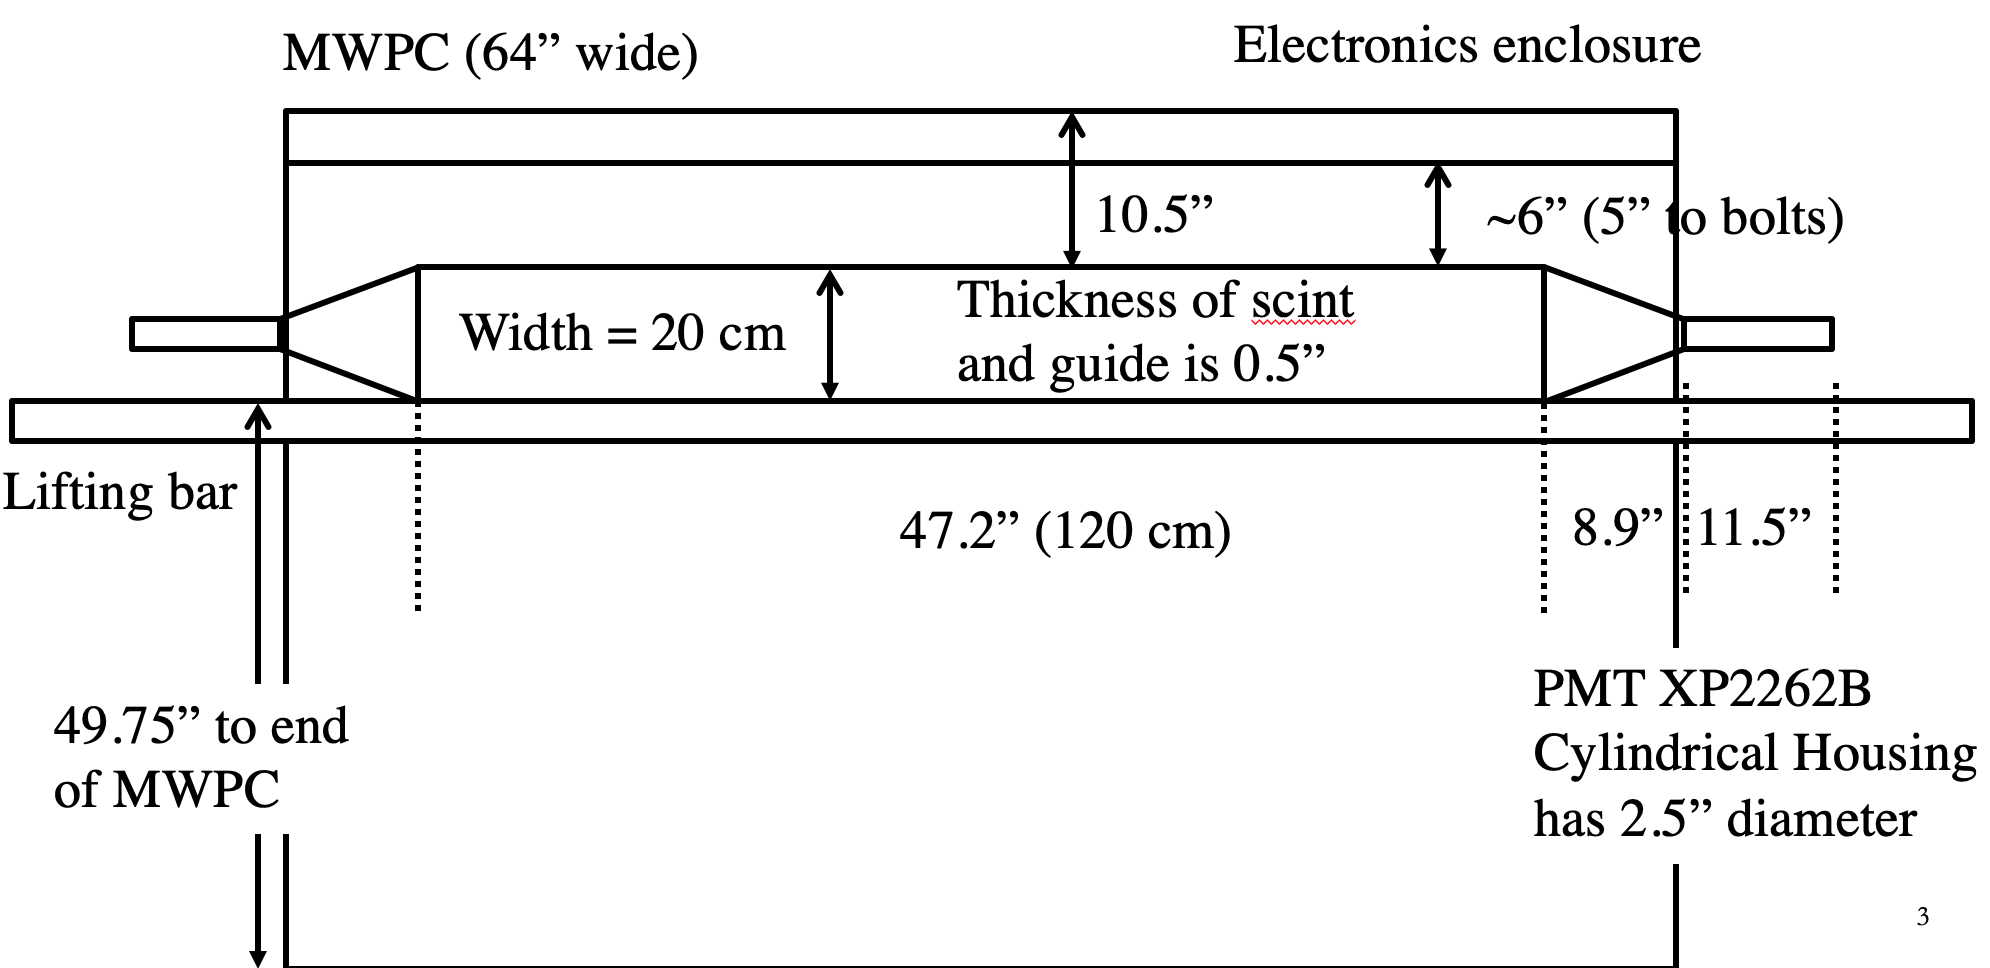
\includegraphics[height=7cm,clip=true]{EEL126_test_plan}
\caption{Top view of the cosmic-ray test setup in EEL 126. The sizes of detectors and relative positions are indicated.
\label{fig:EEL126_test_plan}}
\end{center}
\end{figure} 


\begin{figure}[tbph]
\begin{center}
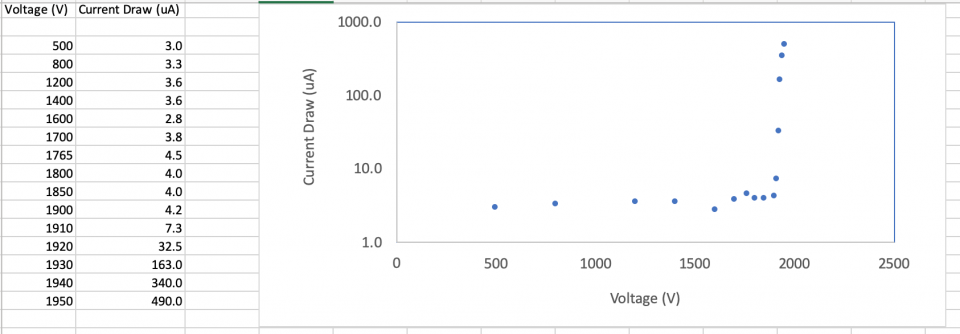
\includegraphics[height=5cm,clip=true]{Current_draw_Frodo}
\caption{Current draw as a function of set voltage for Frodo. The MWPC draws a constant 3-5 $\pm$2$\mu$A up to 1900\,V. The established operating voltage for the chambers is 1765\,V, which corresponds to an approximate gain of $10^5$.
\label{fig:Current_draw_Frodo}}
\end{center}
\end{figure} 

\begin{figure}[tbph]
\begin{center}
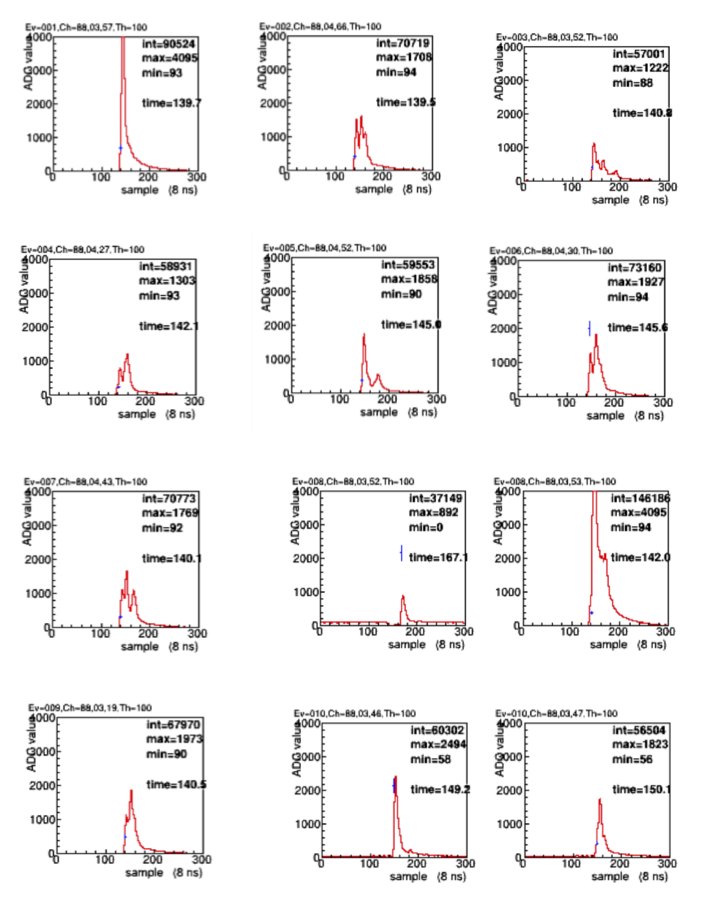
\includegraphics[height=18cm,clip=true]{Waveform_Denethor_R184}
\caption{MWPC Denethor waveforms for the first ten events of R184. The event number is recorded on the top left of each plot. The raw pulse integral and peak values are
also shown for each waveform. Note that for events 8 and 10 there are two adjacent wires hit.  
\label{fig:Waveform_Denethor_R184}}
\end{center}
\end{figure} 

\section{Typical distributions}

\subsection{Scintillators}
Each scintillator is viewed by two XP2262B photomultipliers (PMTs), one at each end. The PMT voltages were set by eye on the scope to deliver similar gain ($\sim$ 30\%). The thresholds were relatively low compared to typical cosmic-ray pulses. Each pulse is required to be within 40 ns of the nominal mean of scintillator hits for the event to be considered in the final analysis. The position along the scintillator can be determined using the time difference between the two PMTs as 
\begin{eqnarray}
x & = & \frac{1}{2} v_{\rm eff} (t_A - t_B),
\end{eqnarray}
where $t_A$ and $t_B$ are the times of the two PMTs and $v_{\rm eff}$= 16.5 cm/ns. Because the scintillators are relatively close together, the position in the top scintillator correlates very strongly with the position in the bottom scintillator as shown in Fig.\,\ref{fig:Scintillator_correlation}. The position resolution along the length of the scintillator is dominated by the 4 ns sampling and the algorithm used to determine the pulse time. As it has little impact on the results here, the algorithm has not been optimized. 
\begin{figure}[tbph]
\begin{center}
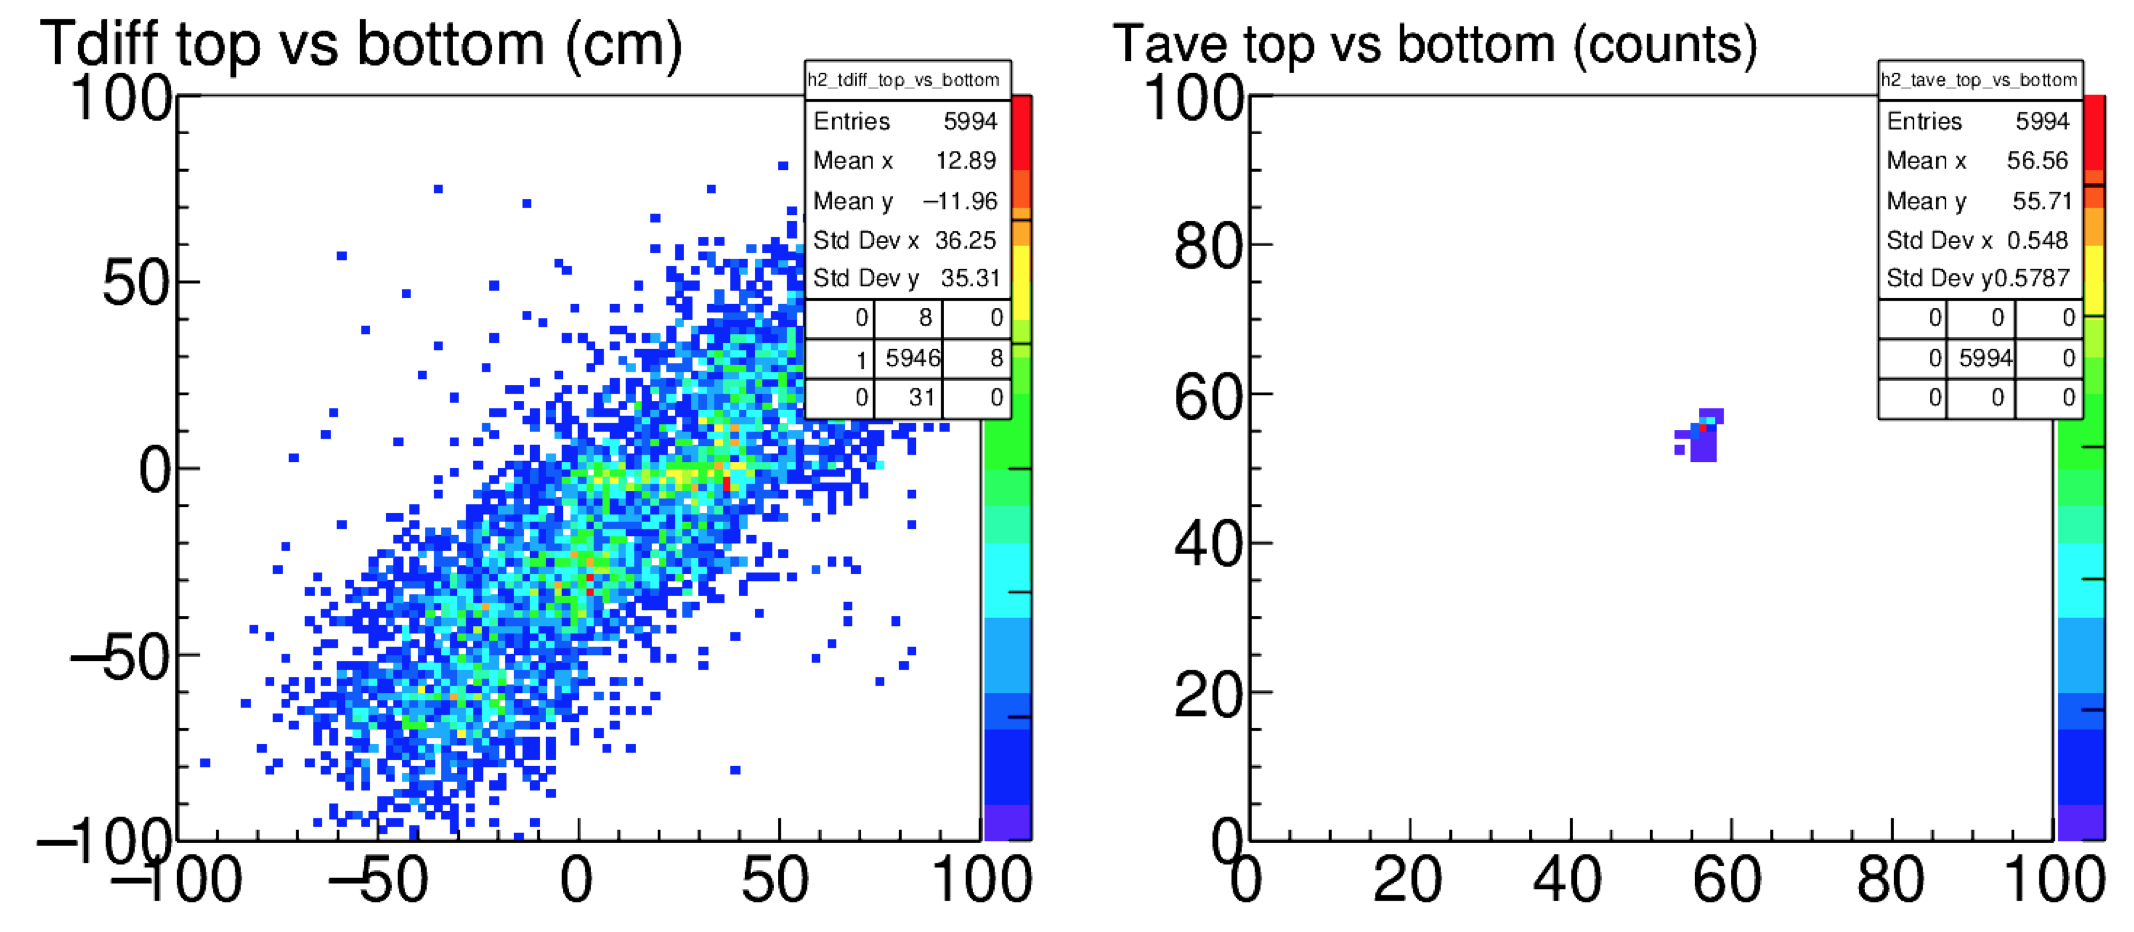
\includegraphics[height=6cm,clip=true]{Scintillator_correlation}
\caption{Left) Correlation between position in the top and bottom scintillators. Right) Average time of PMT times in the top vs the average time in the bottom PMTs. The structures in the correlation plot are a result of the 4\,ns sampling of the waveform.
\label{fig:Scintillator_correlation}}
\end{center}
\end{figure} 

\begin{figure}[tbph]
\begin{center}
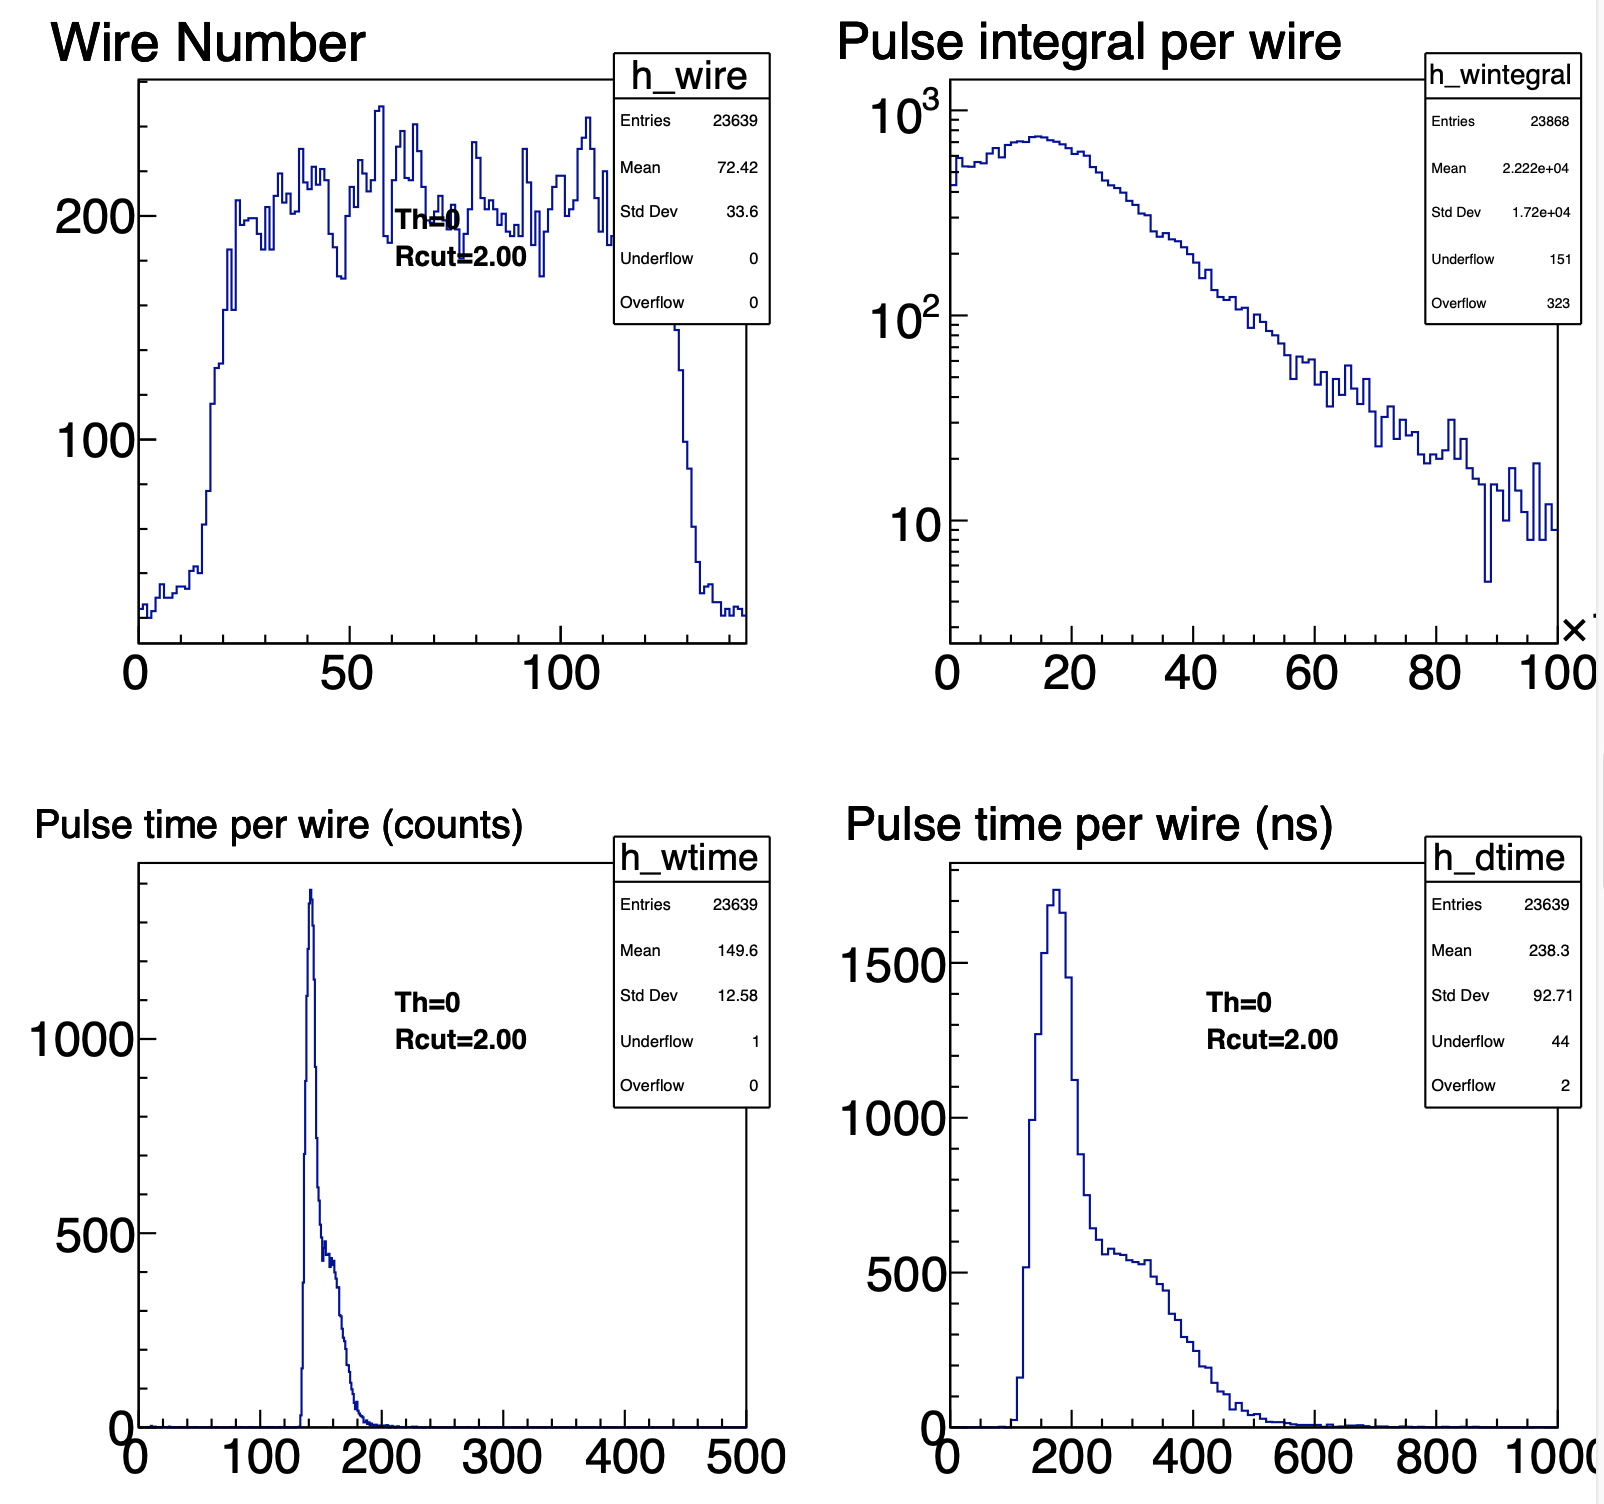
\includegraphics[height=16cm,clip=true]{MWPC_distributions}
\caption{Typical distributions of MWPC distributions plotted for Arwen from 10,000 events from R188. Top left) Wire occupancy plot. The central region is illuminated by the scintillators; the edges show cosmic-ray hits from showers in coincidence with the trigger. Top right) Distribution of the pedestal-subtracted waveform integral on a logarithmic scale. Note that the x-axis is in units of $10^3$ integral counts. Bottom left) Drift time distribution in FADC counts. Bottom right) Selection of drift time region converted to ns. Note that there are essentially no hits outside the drift time interval.
\label{fig:MWPC_distributions}}
\end{center}
\end{figure} 


\begin{figure}[tbph]
\begin{center}
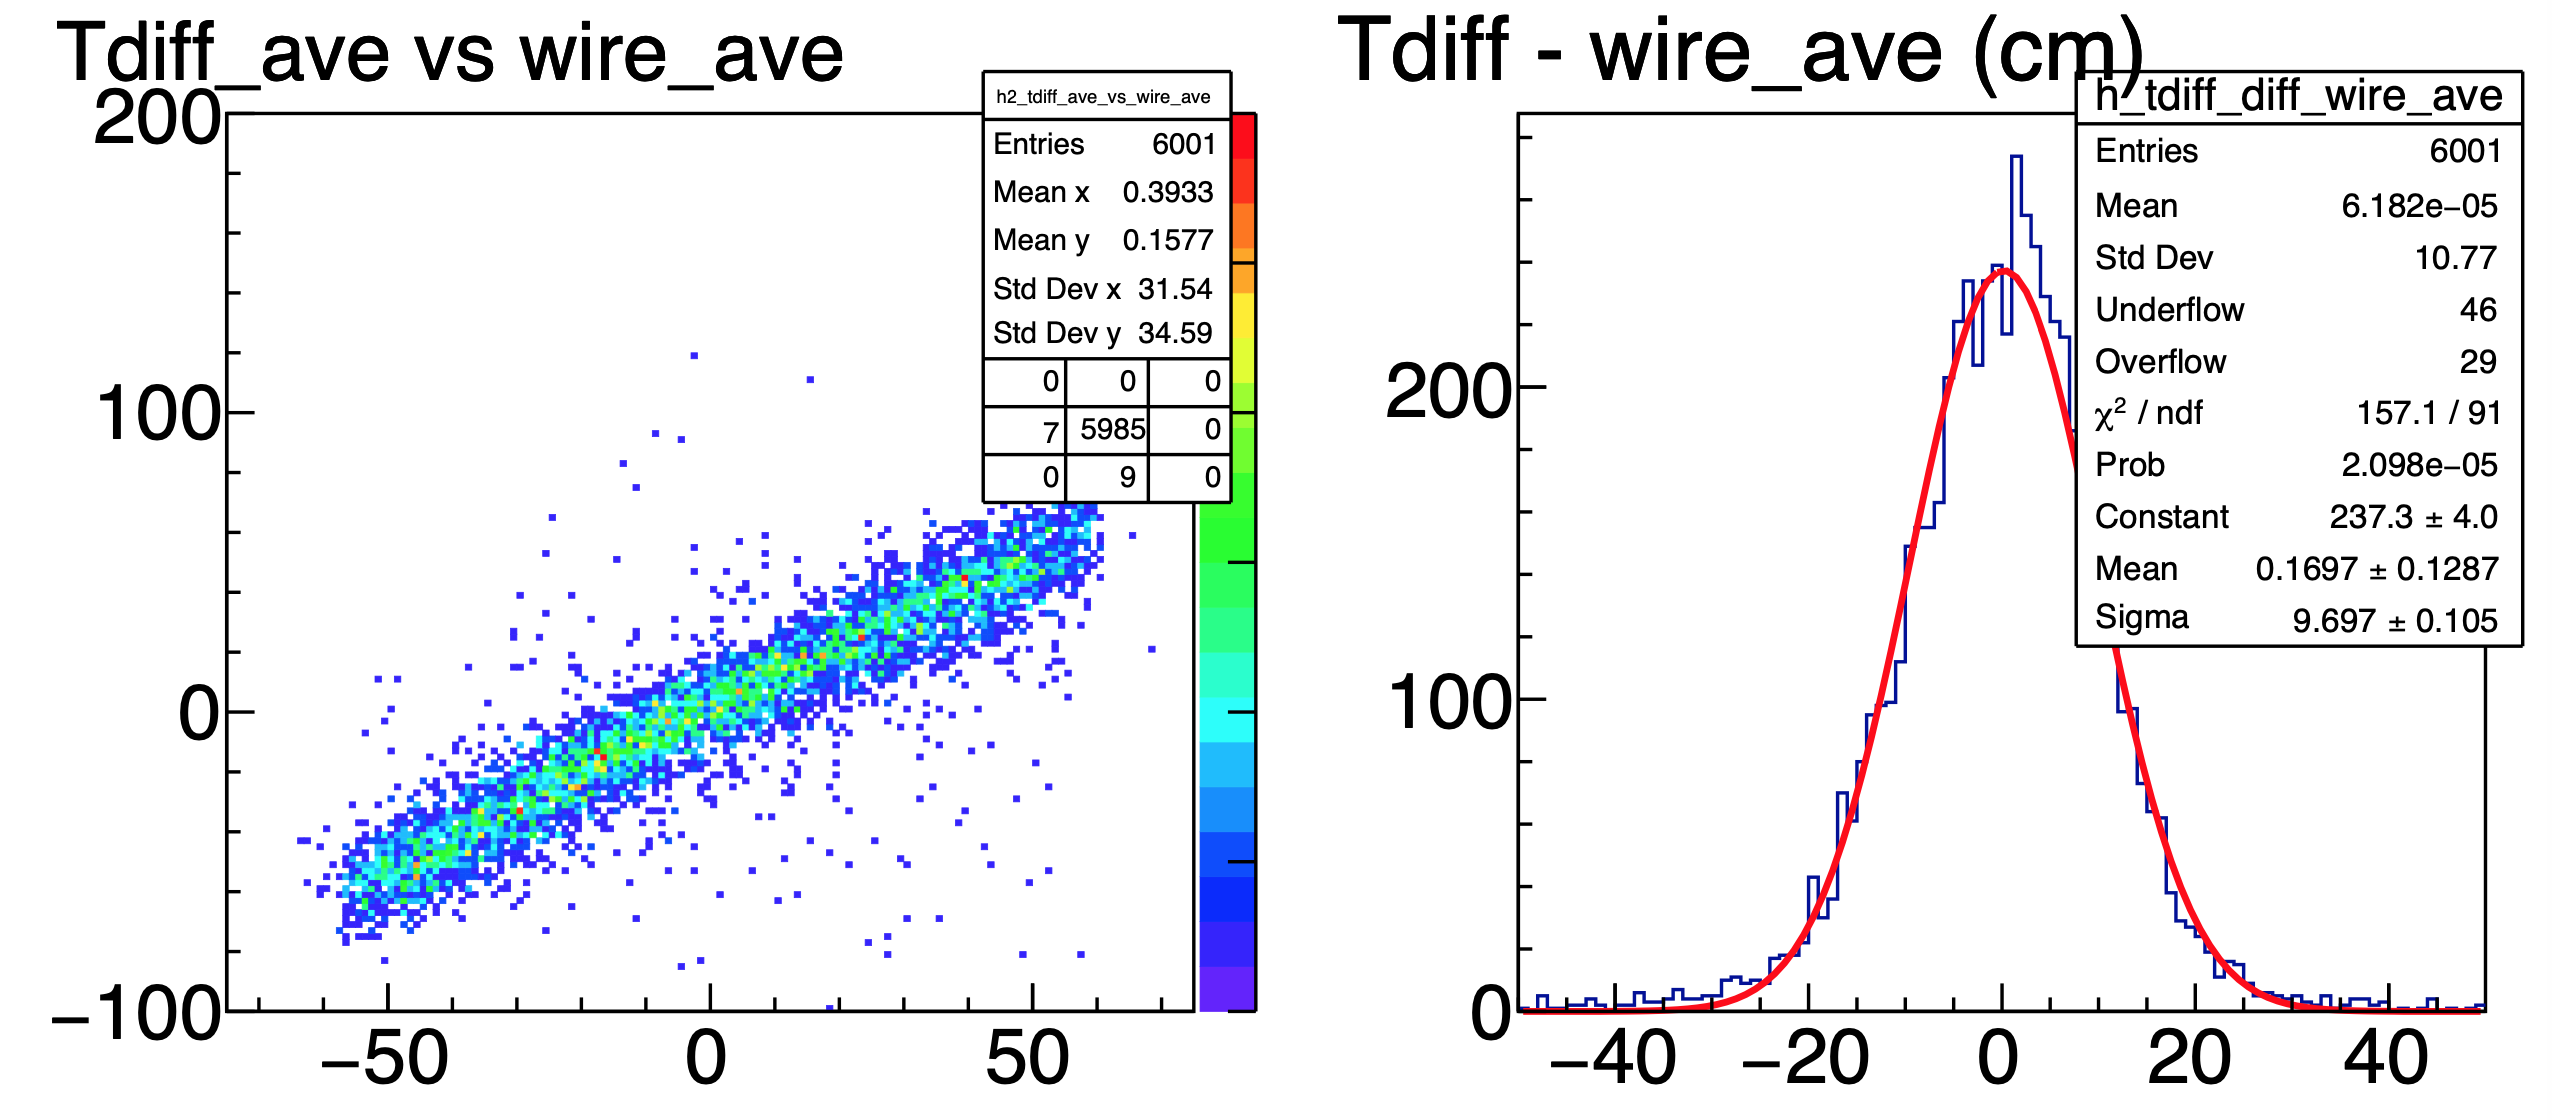
\includegraphics[height=6cm,clip=true]{MWPC_scint_correlation}
\caption{Left) Correlation between the average of the position in the top and bottom scintillators versus the average number of the hit wires. Right) Histogram of the difference between the average scintillator position and the average wire number. The width of 9.7 cm is consistent with the scintillator resolution dominated by the 4\,ns sampling.
\label{fig:MWPC_scint_correlation}}
\end{center}
\end{figure} 

\begin{figure}[tbph]
\begin{center}
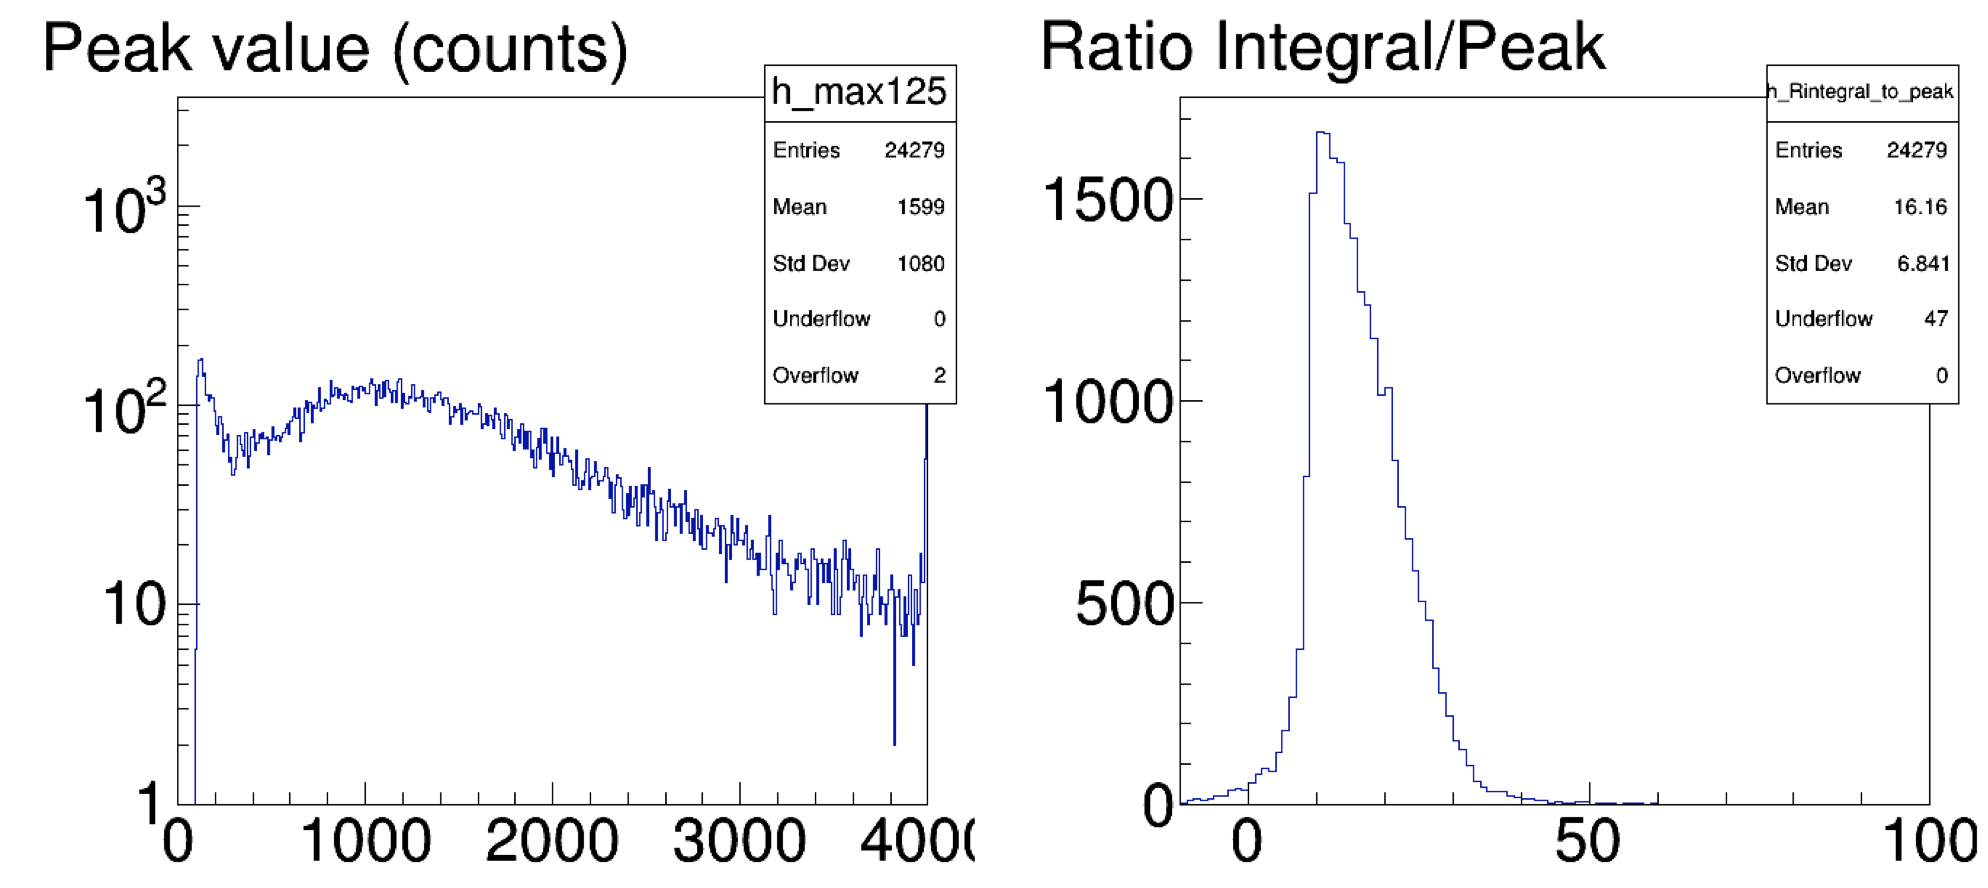
\includegraphics[height=6.5cm,clip=true]{Rint_to_peak}
\caption{Left) Peak value above pedestal. Right) Ratio of pedestal-subtracted integral over peak. Pulses with small or negative values of the ratio are indicative of oscillatory electronic noise.
\label{fig:Rint_to_peak}}
\end{center}
\end{figure} 



\begin{figure}[tbph]
\begin{center}
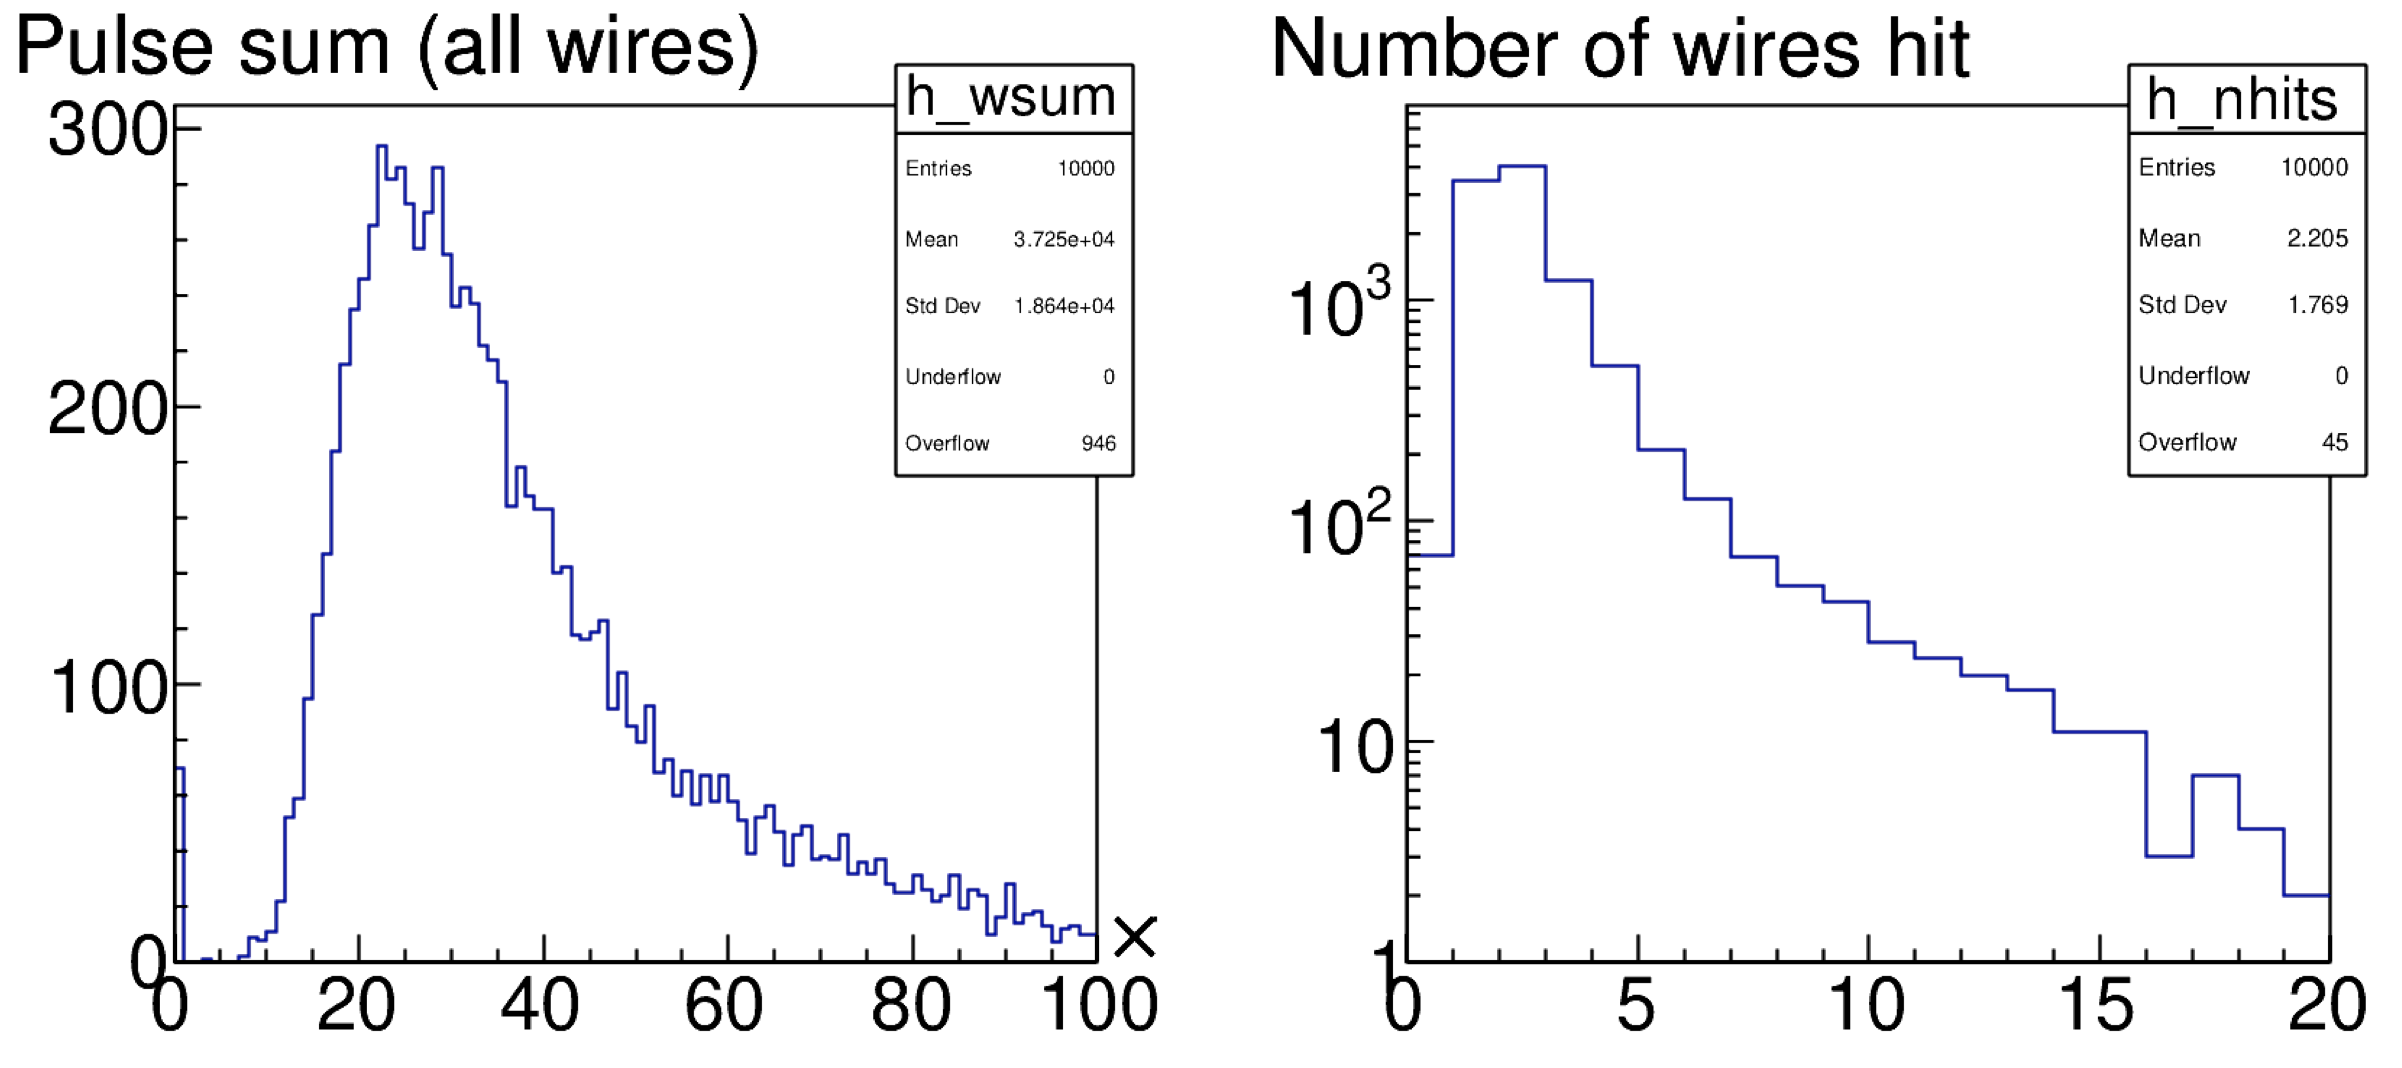
\includegraphics[height=6.5cm,clip=true]{Arwen_R188_sum_nhits}
\caption{Distributions for all triggers, not selected for cuts on scintillator hits.
Left) Wire sum of all pulse integrals per event. Right) Raw distribution of number of hits per event.
\label{fig:Arwen_R188_sum_nhits}}
\end{center}
\end{figure} 

\subsection{MWPCs}
Examples of the waveforms for the MWPCs are shown in Fig.\,\ref{fig:Waveform_Denethor_R184}. The pulses are quite large relative to the baseline and for the most part we use the pulses found in the firmware emulation that determines pulse parameters \cite{hdnote2274}. We are currently running in mode 6 ``CDC\_long,'' which reads out the full waveform from the flash ADCs, as well as the pulse parameters determined by the firmware.  The default algorithm uses a threshold of 100 counts above threshold to find pulses (see Fig.~1 in the reference). In Fig.\,\ref{fig:MWPC_distributions} we show a typical occupancy plot, pulse integral distribution as well as the drift time. The distributions of the sum of all pulses integrals in one event and the distribution of number of hits are shown in Fig.\,\ref{fig:Arwen_R188_sum_nhits}.
The correlation between the position as determined by the scintillators and the wire number can be seen in Fig.\,\ref{fig:MWPC_scint_correlation}. The width of the distribution is dominated by the scintillator resolution. The firmware also reports the peak value of the waveform and the ratio $R_{\rm int}= (integral - pedestal)/(peak-pedestal)$ that is a useful quantity to distinguish noise from signal. See Fig.\,\ref{fig:Rint_to_peak}. For a constant signal shape, $R_{\rm int}$ is a constant, and any oscillatory behavior of the baseline tends to average to zero.  For the analysis, we require $R_{\rm int} > R_{\rm cut} =2$, which has little effect on the final answers, but does eliminate some electronic noise from the analysis. 

\section{Efficiencies \label{sec:eff}}
In order to estimate the chamber efficiencies, we sum pulse integrals (above pedestal) for all wires that have a found pulse for a given trigger. We use a sample of 10k triggered events for each measurement. For all chambers but Frodo and Galadriel (See discussion in Section\,\ref{sec:noise}), the sum is essentially the raw sum of pulses provided by the firmware. The efficiency for each MWPC is estimated by taking events above a software threshold on the sum of pulses. Events below the threshold constitute the inefficiency, as plotted as a function of the threshold in Figs.\,\ref{fig:efficiencies_a-d} and \ref{fig:efficiencies_e-f}. We find that the efficiencies are above 99.7\% up to thresholds on the sum of about 8,000 integrated counts. For a typical ratio $R_{\rm int}$ of 10.7, this corresponds to keeping pulses with peak values greater than 750 counts above pedestal. The efficiency measurement covers the central region of the chamber (approximately wires 16-128 out of 144). 

We have performed a voltage scan on two of the MWPCs (Arwen and Denethor) to determine the sensitivity of these measurements to the nominal gain setting of HV=1765\,V.  The applied high voltage ranged from HV=1690 to 18140\,V. The wire sum distribution and plot of inefficiency vs threshold can be found in 
Fig.\,\ref{fig:Denethor_HV1690_HV1815} 
for Denethor at HV=1690 and 1815\,V. The chamber performs quite well over this entire voltage range of 125\,V. The efficient range of software thresholds on the wire sum distribution is reduced, but still represents a very clear region region to establish a working threshold. One can use the number of MWPC hits per 10k triggers to determine a plateau curve, as shown in Fig.\,\ref{fig:plot_HVscan}. We plot the number of MWPC hits and gain relative to their value at the nominal voltage of HV=1765\,V as a function of voltage. The rates are quite flat, even as the gain varies by a factor of six. We see that the rate starts to increase above 1800\,V. The noise levels in the chambers begin to increase and this can be seen in the deterioration of the typical distributions that validate the MWPC performance. In  Fig.\,\ref{fig:Denethor_R183_HV1840_Th200} 
we show the drift time distribution and correlation between scintillators and MWPC hits for the run at HV=1840\,V. One can clearly see random hits appearing in the drift time distribution as well as hits that do not correlate well between the position determined by the scintillator and the average wire number hit. Compare these distributions with those for the nominal voltage in Figs.\,\ref{fig:MWPC_distributions} and \ref{fig:MWPC_scint_correlation}. For voltages below about 1800\,V, there are no apparent differences between these measured distributions to the ones obtained at nominal voltage. 

\begin{figure}[tbph]
\begin{center}
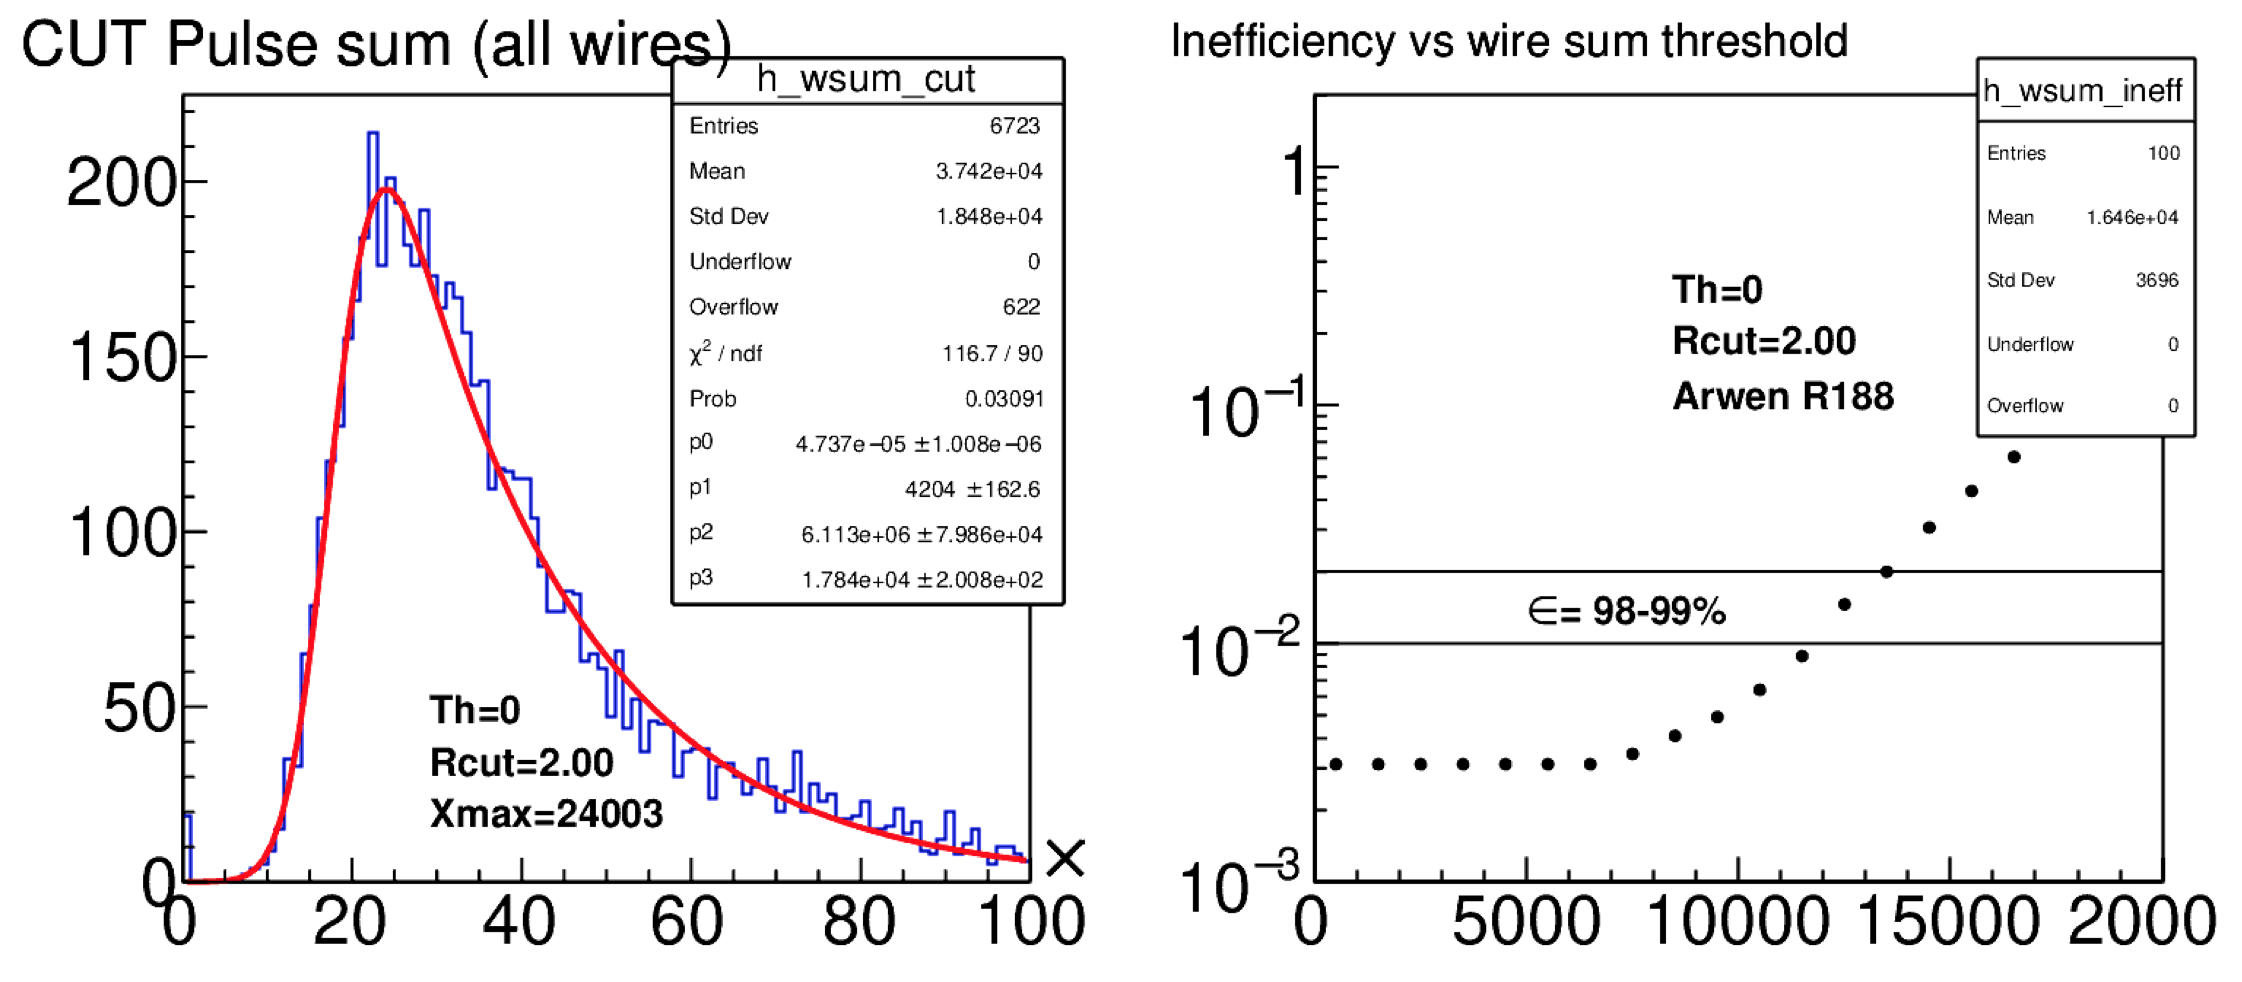
\includegraphics[height=5cm,clip=true]{Arwen_R188_eff}
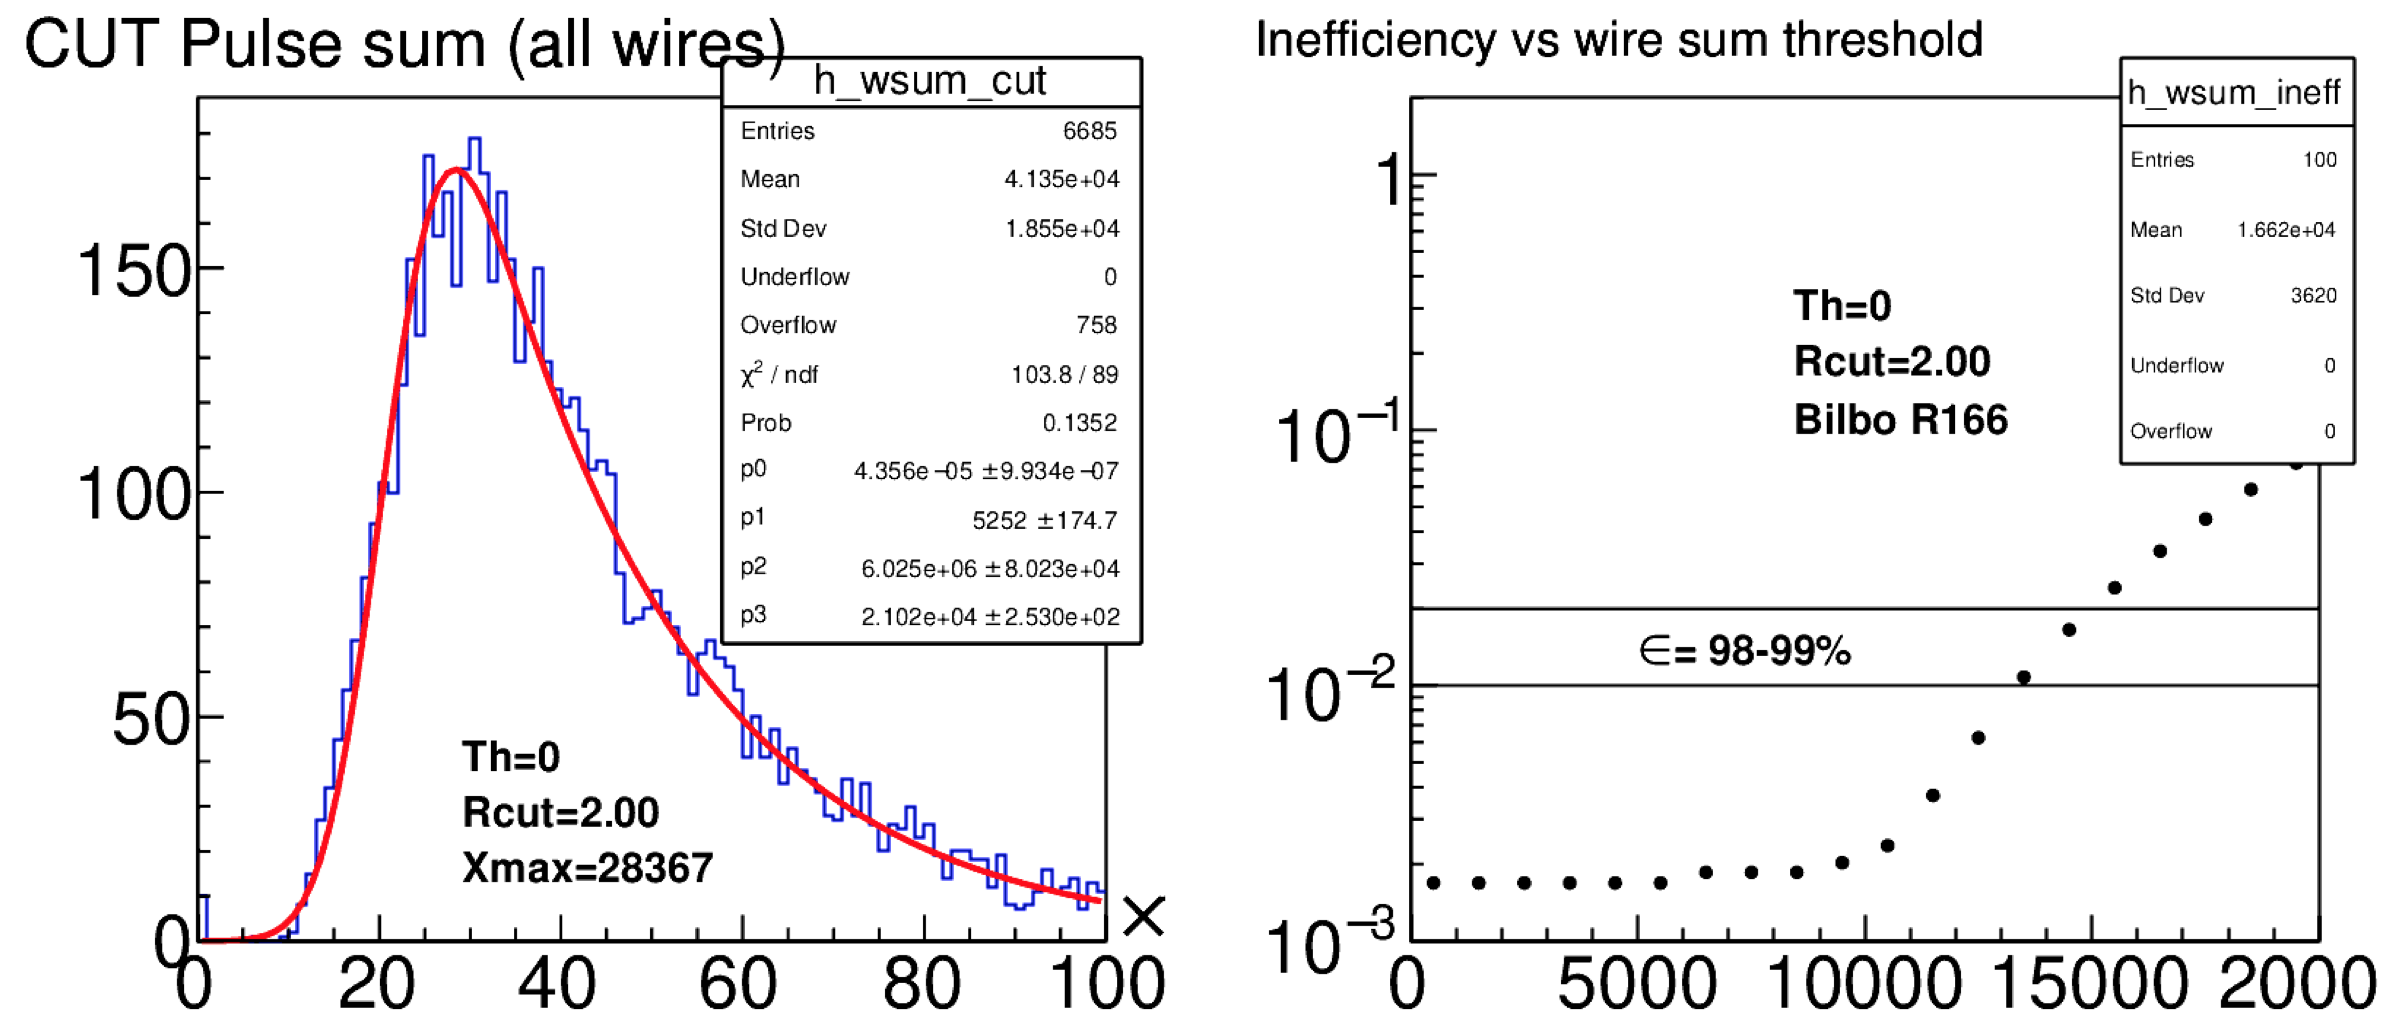
\includegraphics[height=5cm,clip=true]{Bilbo_R166_eff}
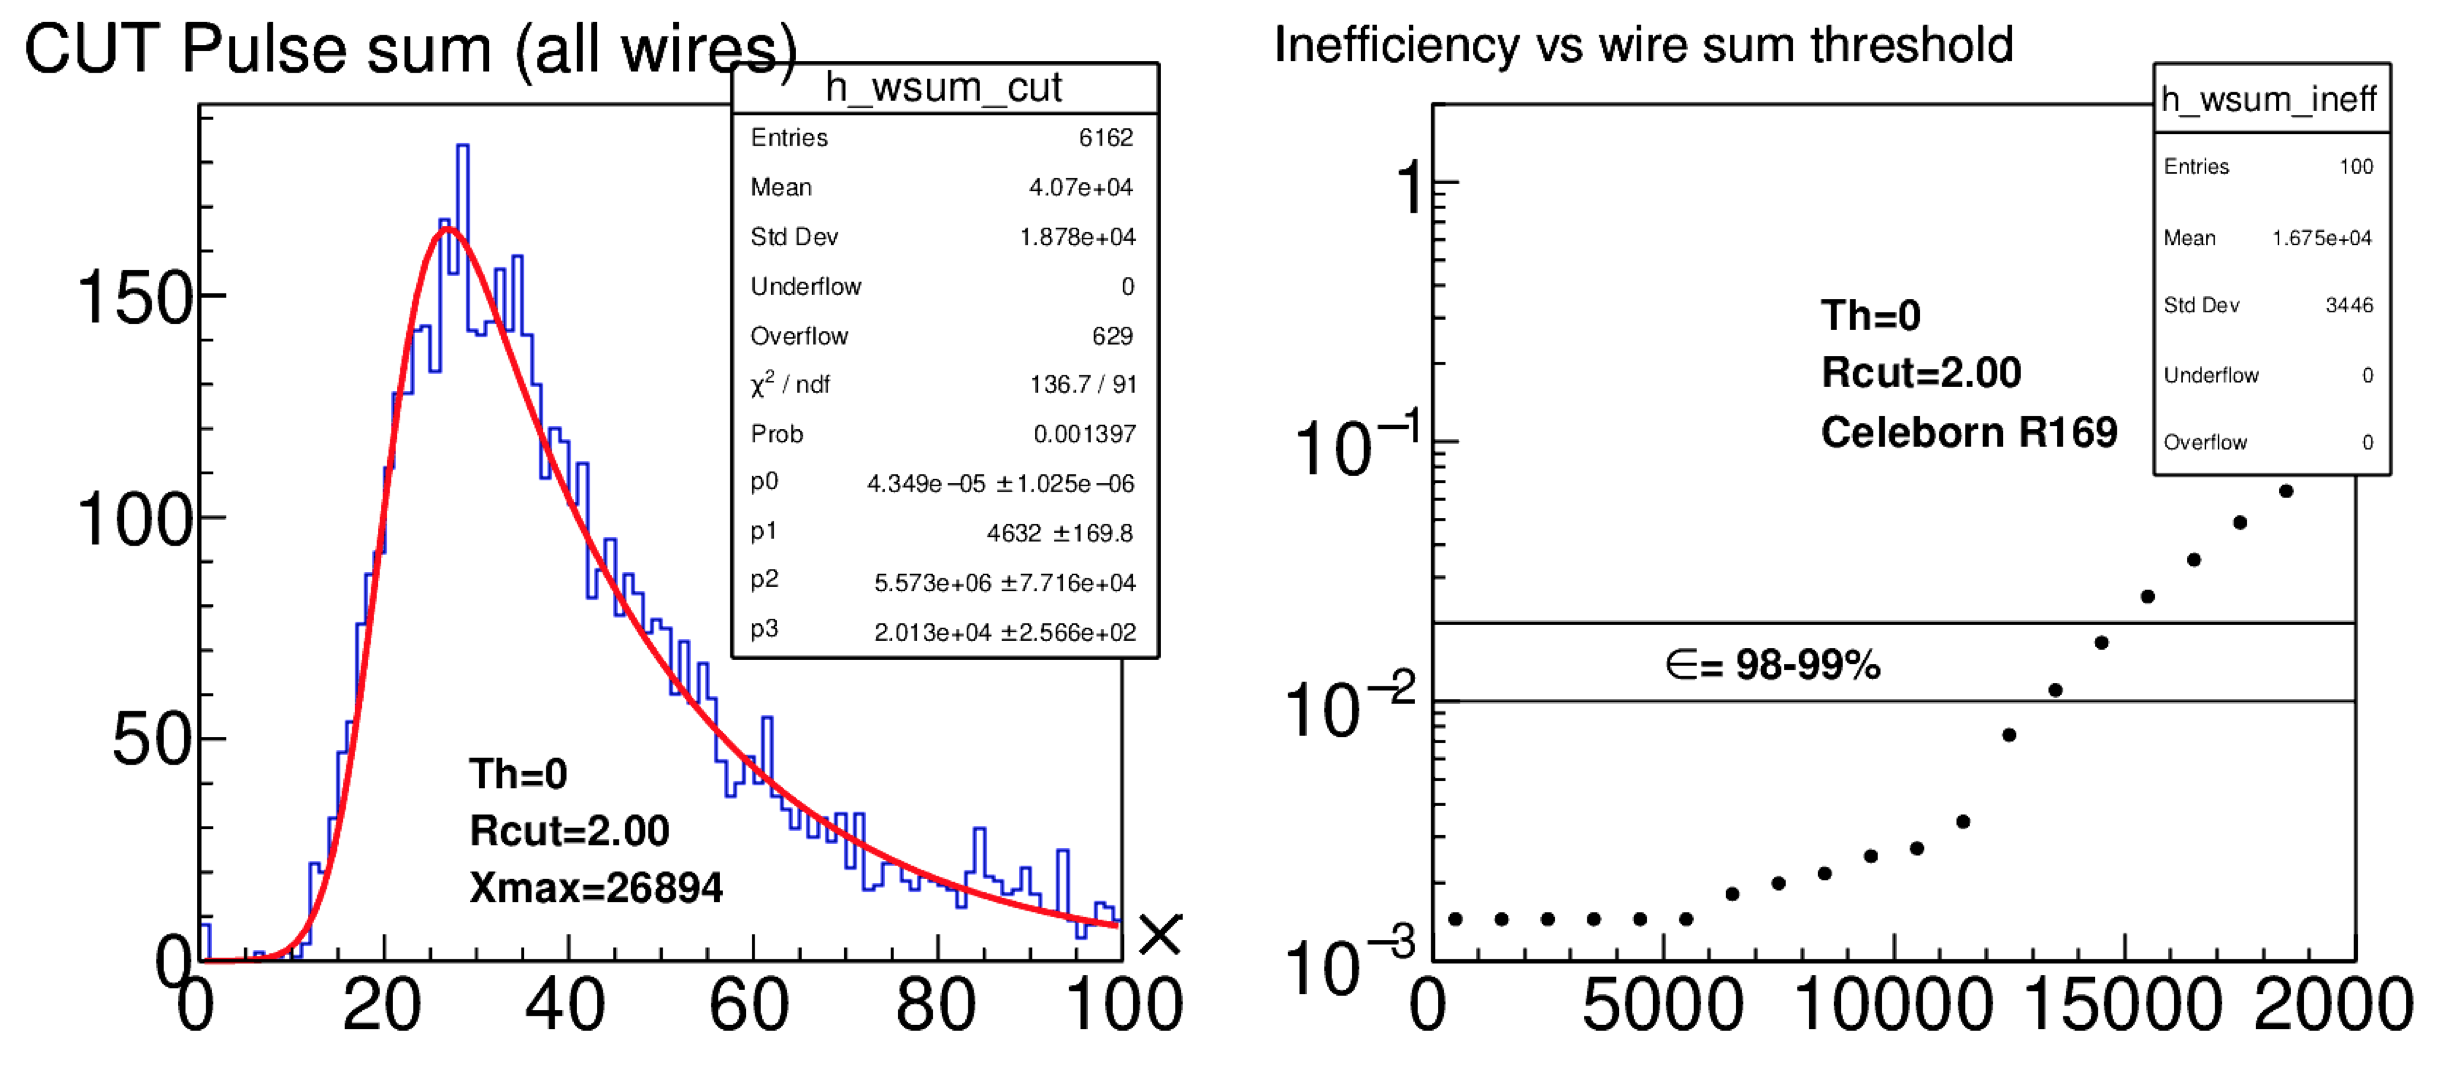
\includegraphics[height=5cm,clip=true]{Celeborn_R169_eff}
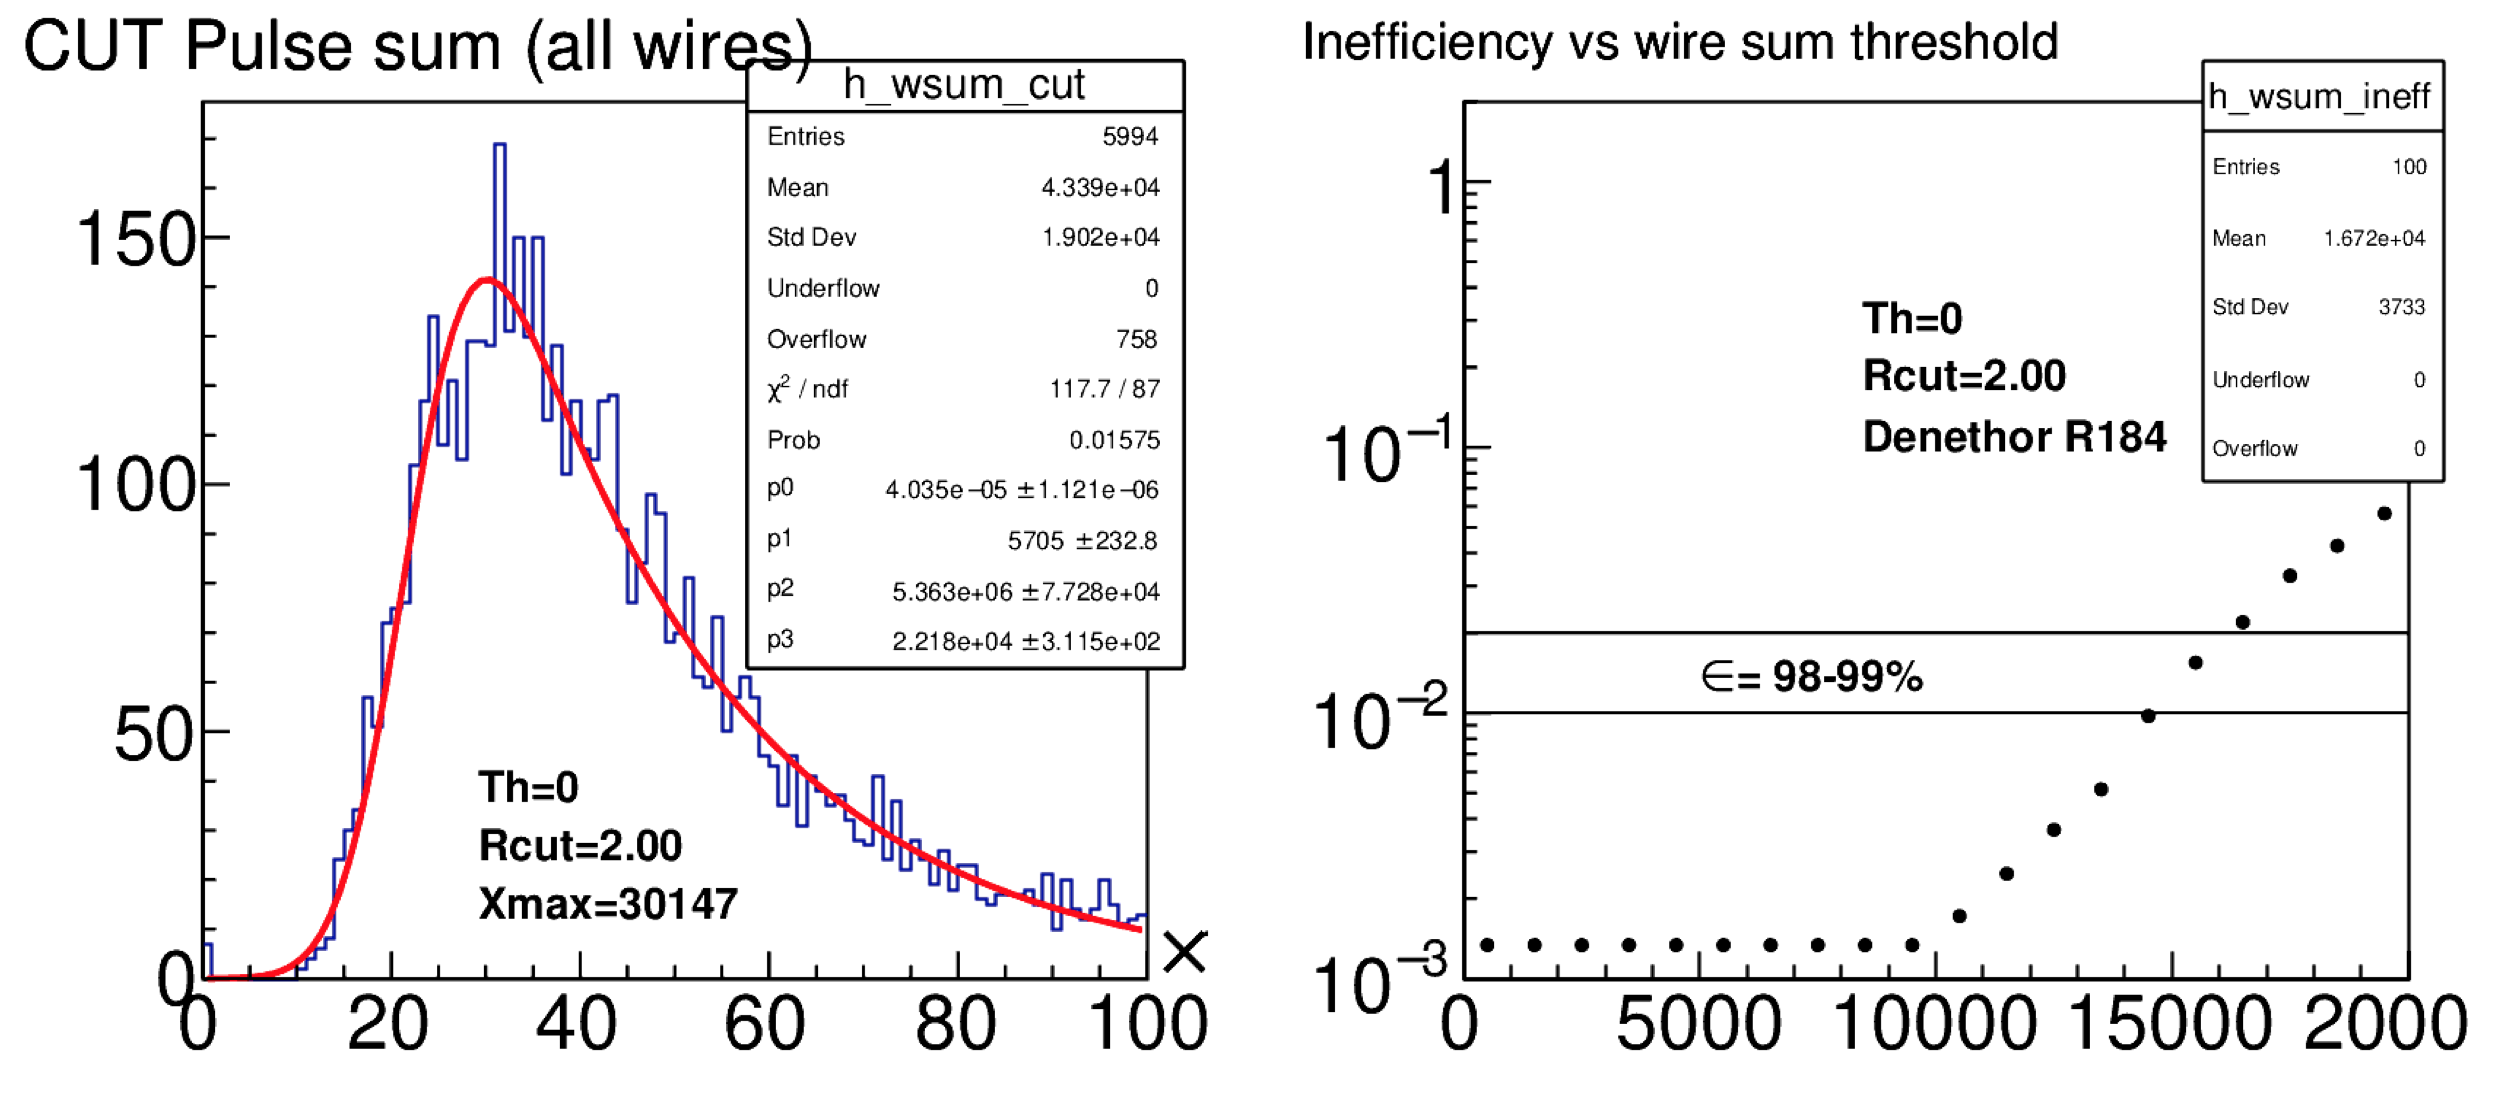
\includegraphics[height=5cm,clip=true]{Denethor_R184_eff}
\caption{Top to Bottom: Arwen, Bilbo, Celeborn and Denethor. Left column) Sum of wire integrals. The x-axis is scaled by $10^3$. Right) Inefficiency estimate vs threshold.
\label{fig:efficiencies_a-d}}
\end{center}
\end{figure} 

\begin{figure}[tbph]
\begin{center}
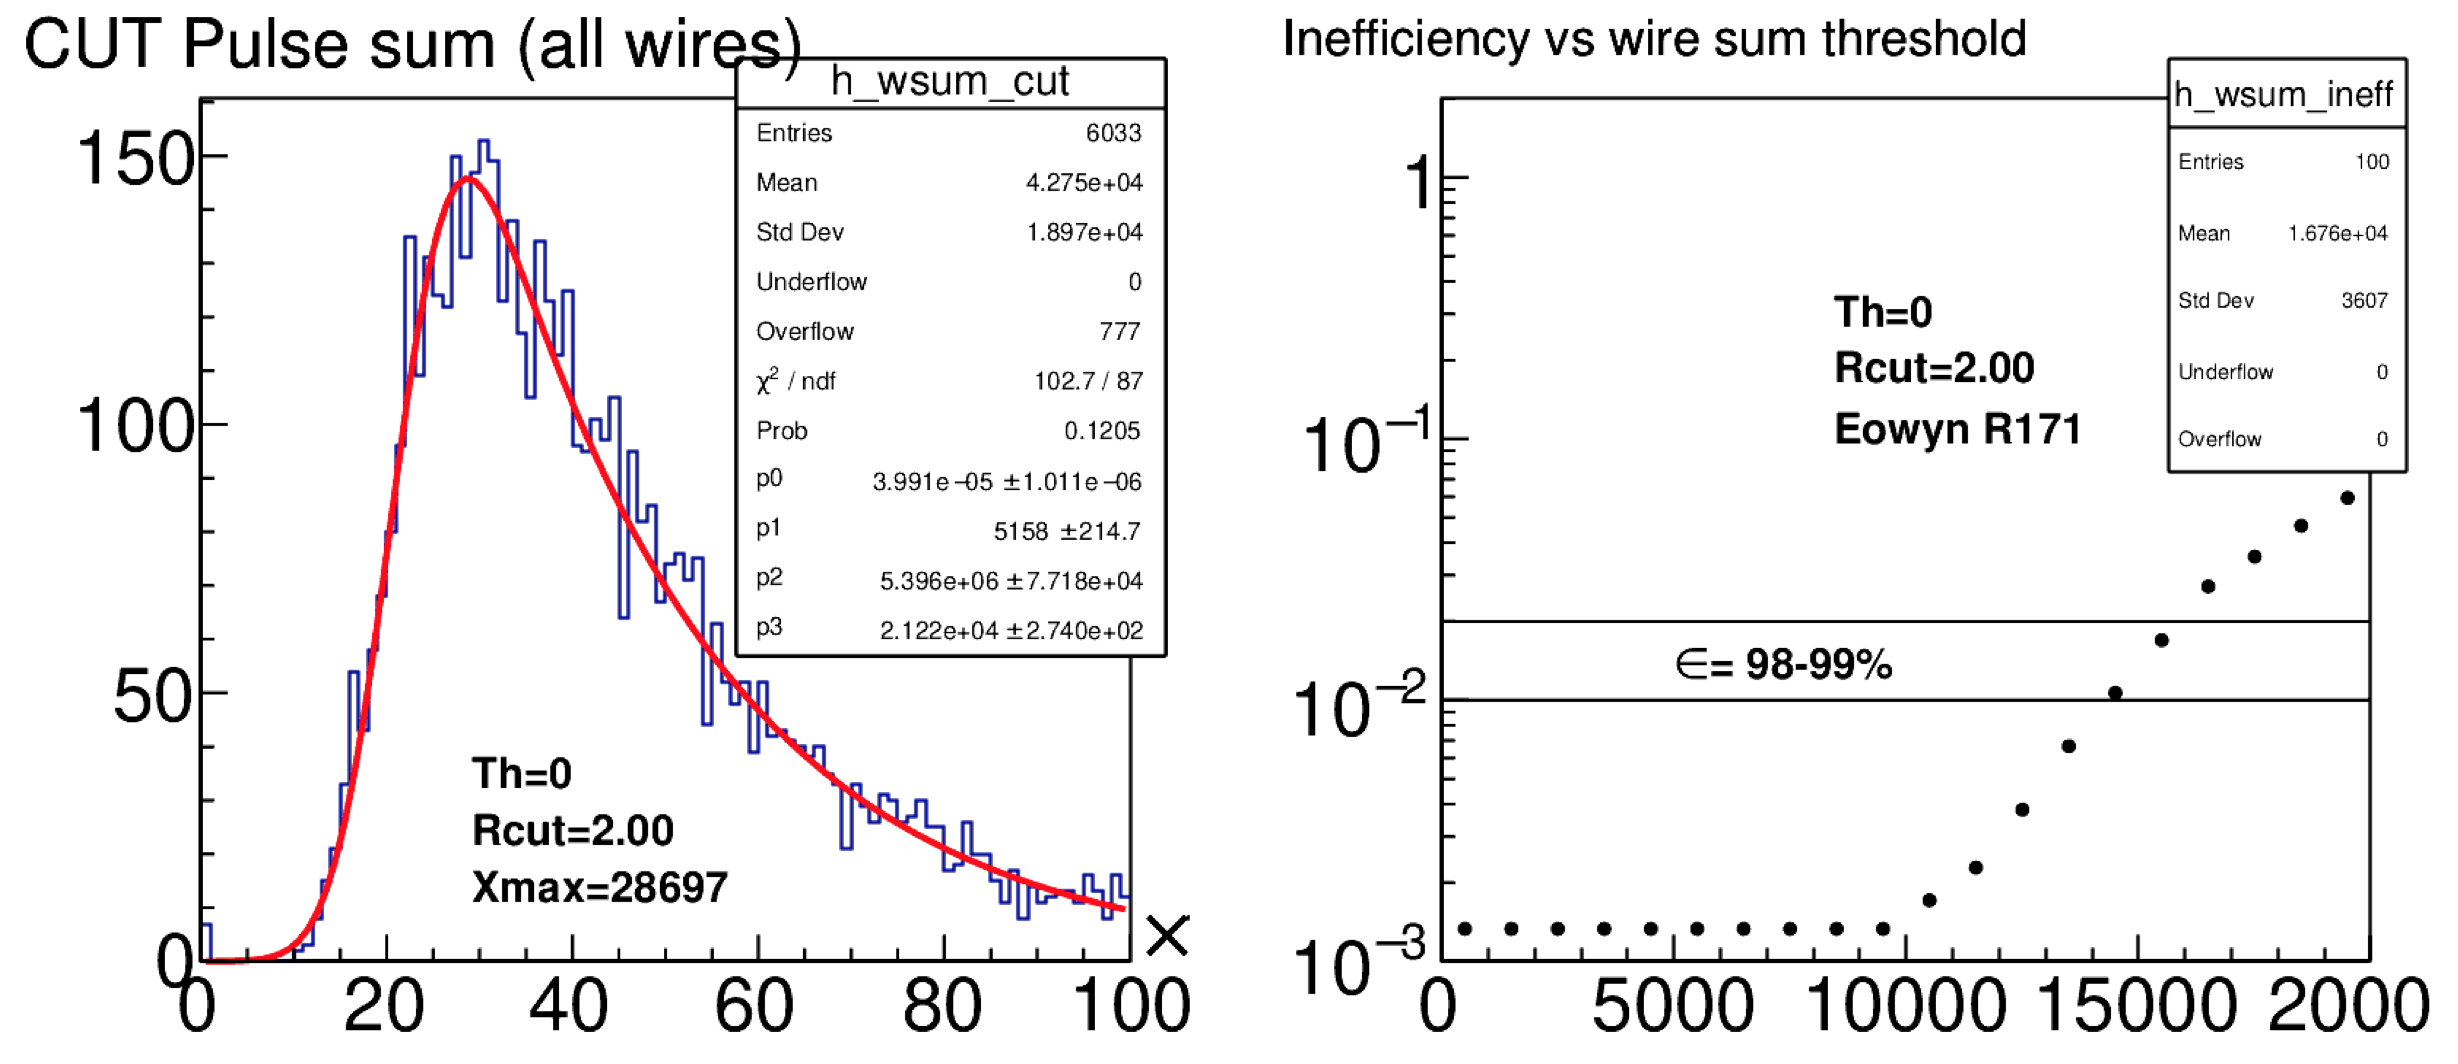
\includegraphics[height=5cm,clip=true]{Eowyn_R171_eff}
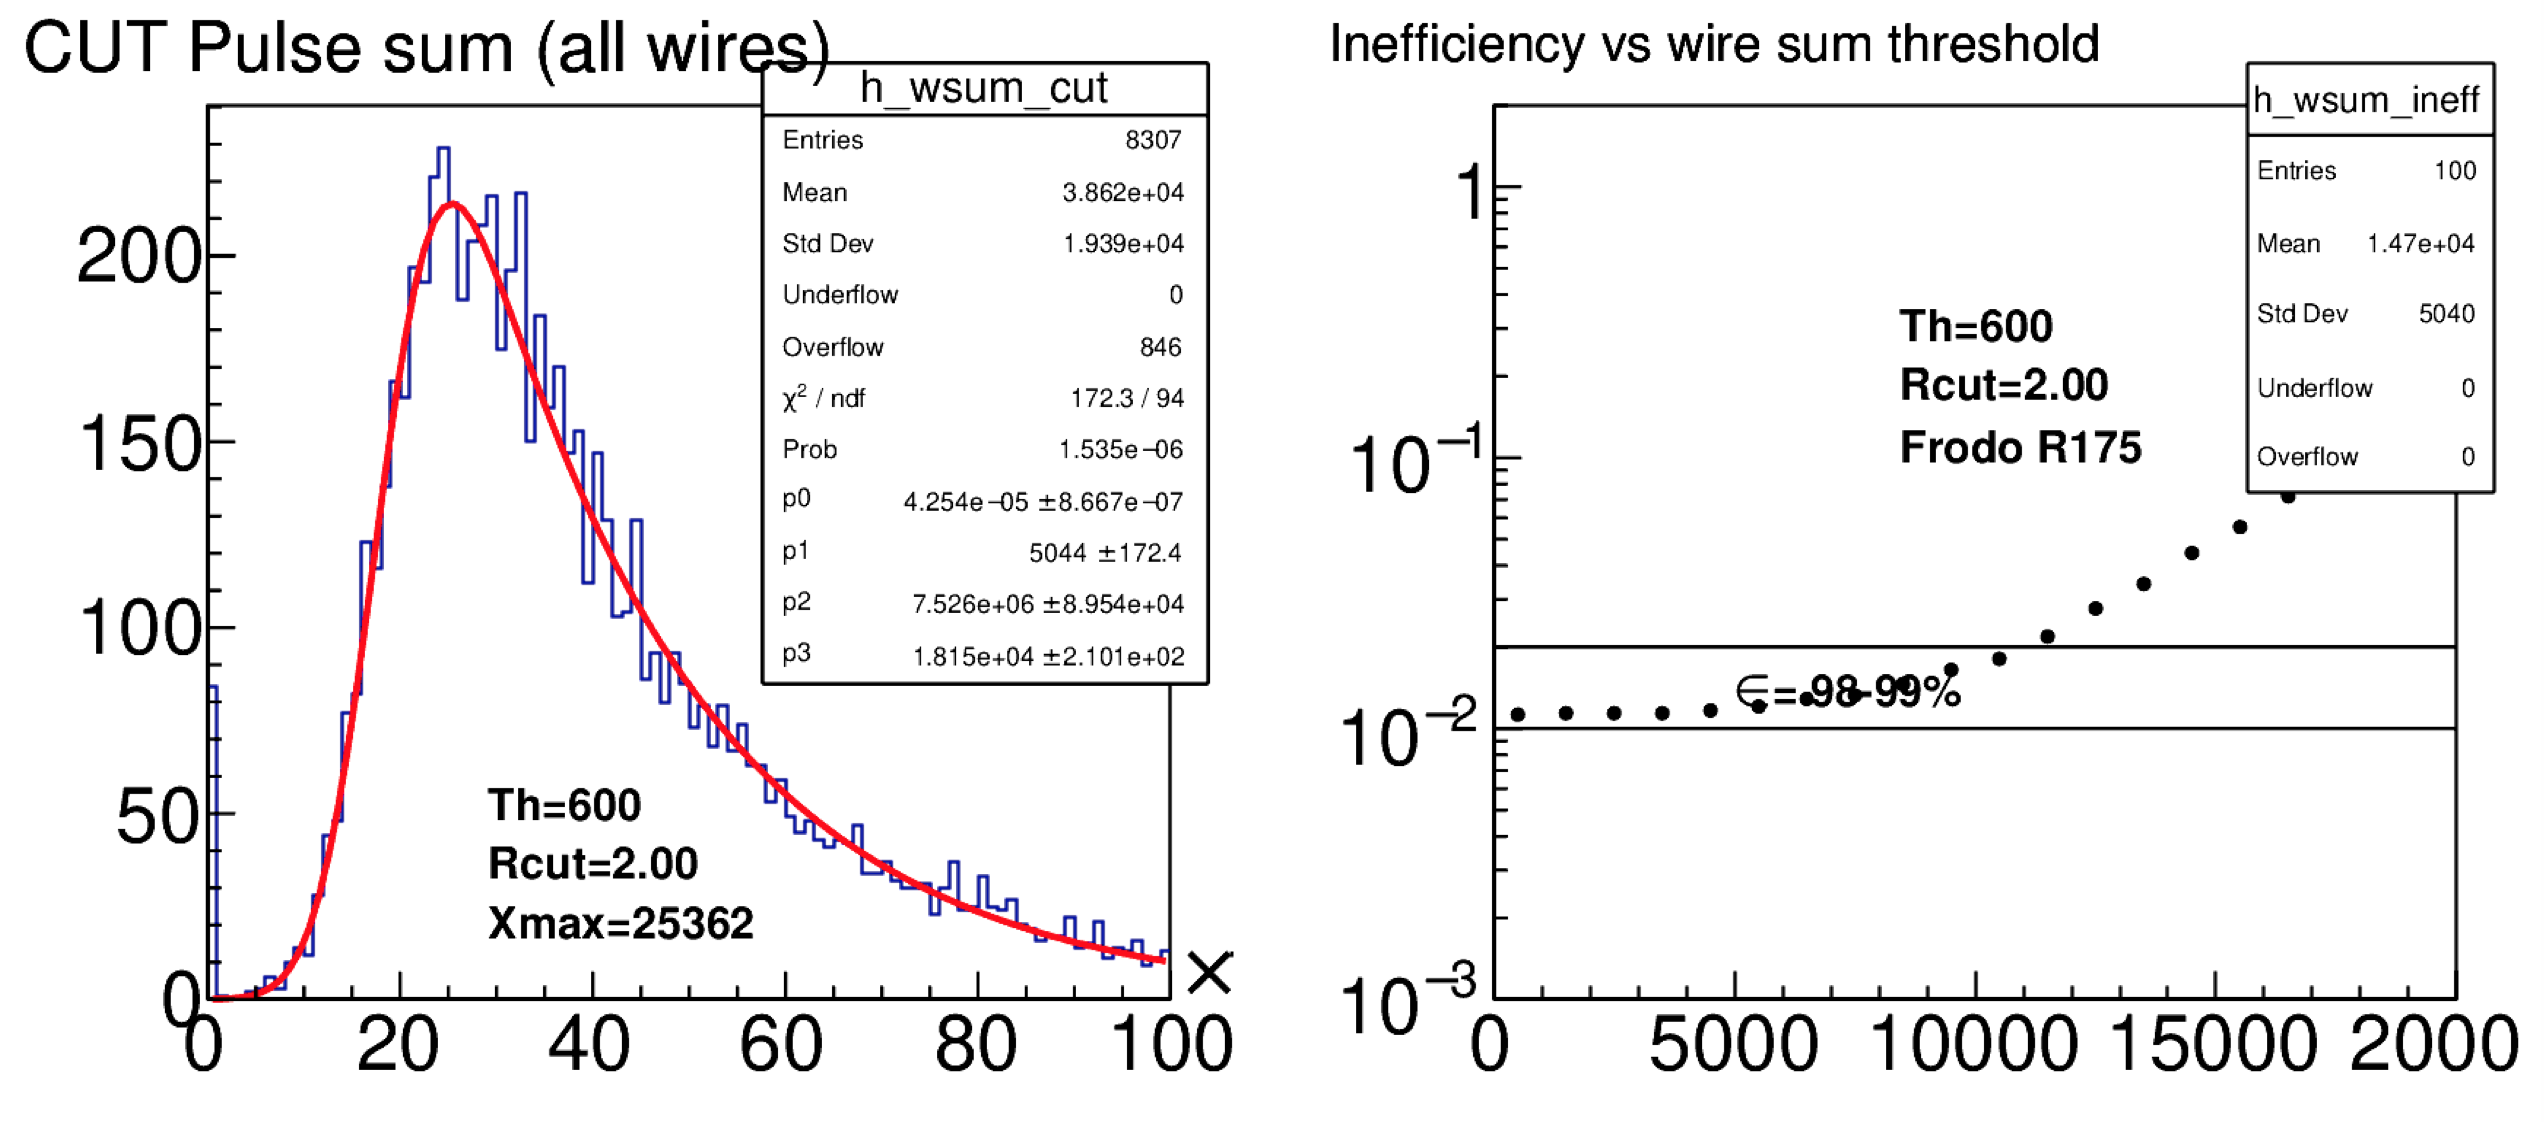
\includegraphics[height=5cm,clip=true]{Frodo_R175_Th600_eff}
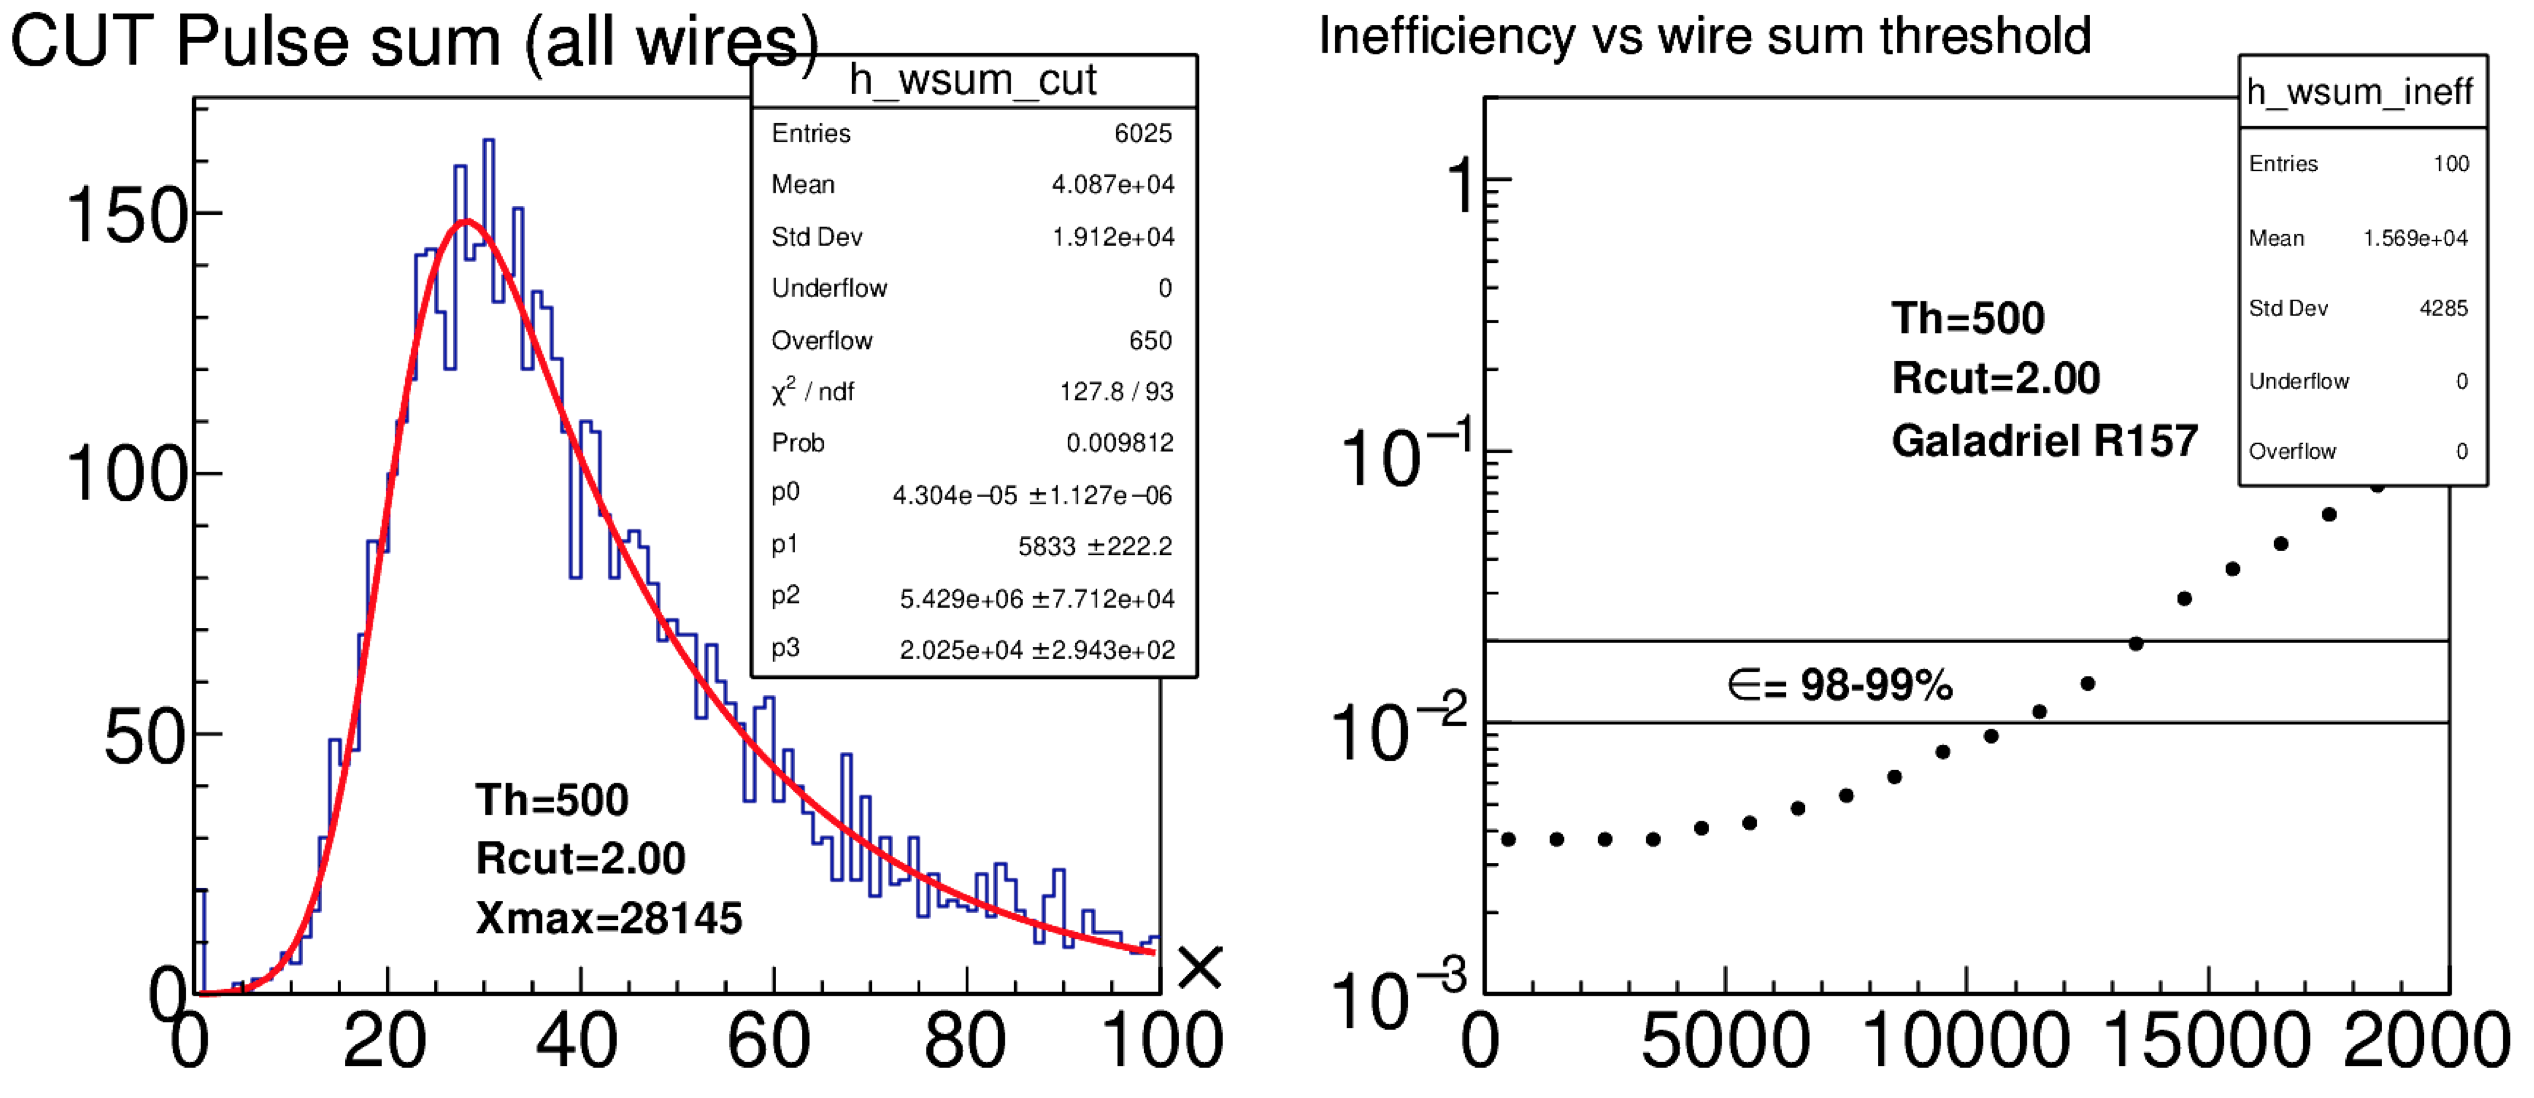
\includegraphics[height=5cm,clip=true]{Galadriel_R157_Th500_eff}
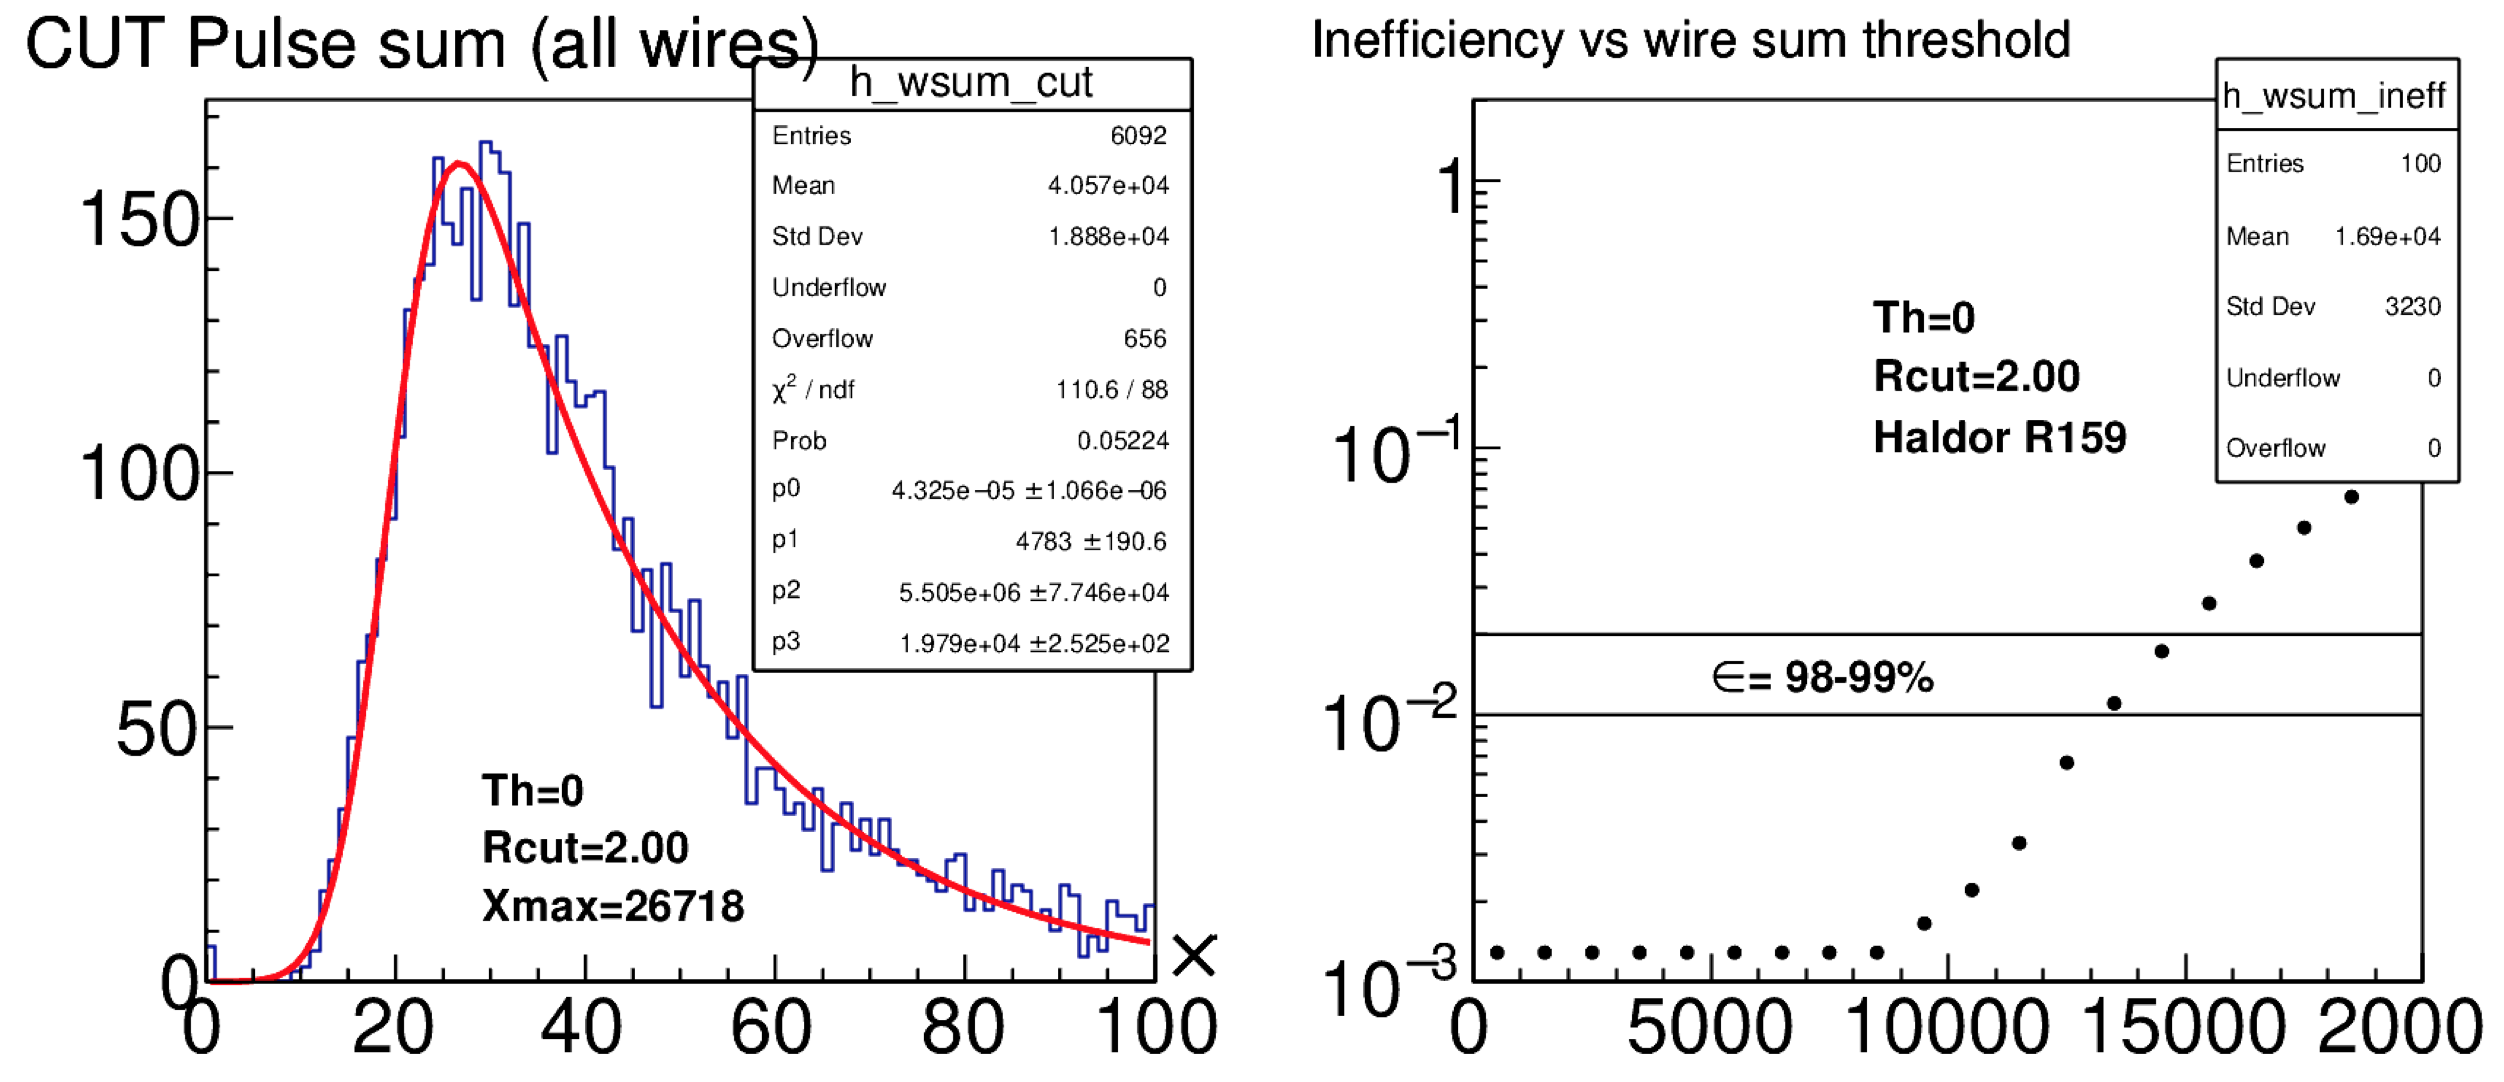
\includegraphics[height=5cm,clip=true]{Haldor_R159_eff}
\caption{Top to Bottom: Eowyn, Frodo (Th=600), Galadriel (Th=500) and Haldor. Left column) Sum of wire integrals. The x-axis is scaled by $10^3$. Right) Inefficiency estimate vs threshold.
\label{fig:efficiencies_e-f}}
\end{center}
\end{figure} 


\begin{figure}[tbph]
\begin{center}
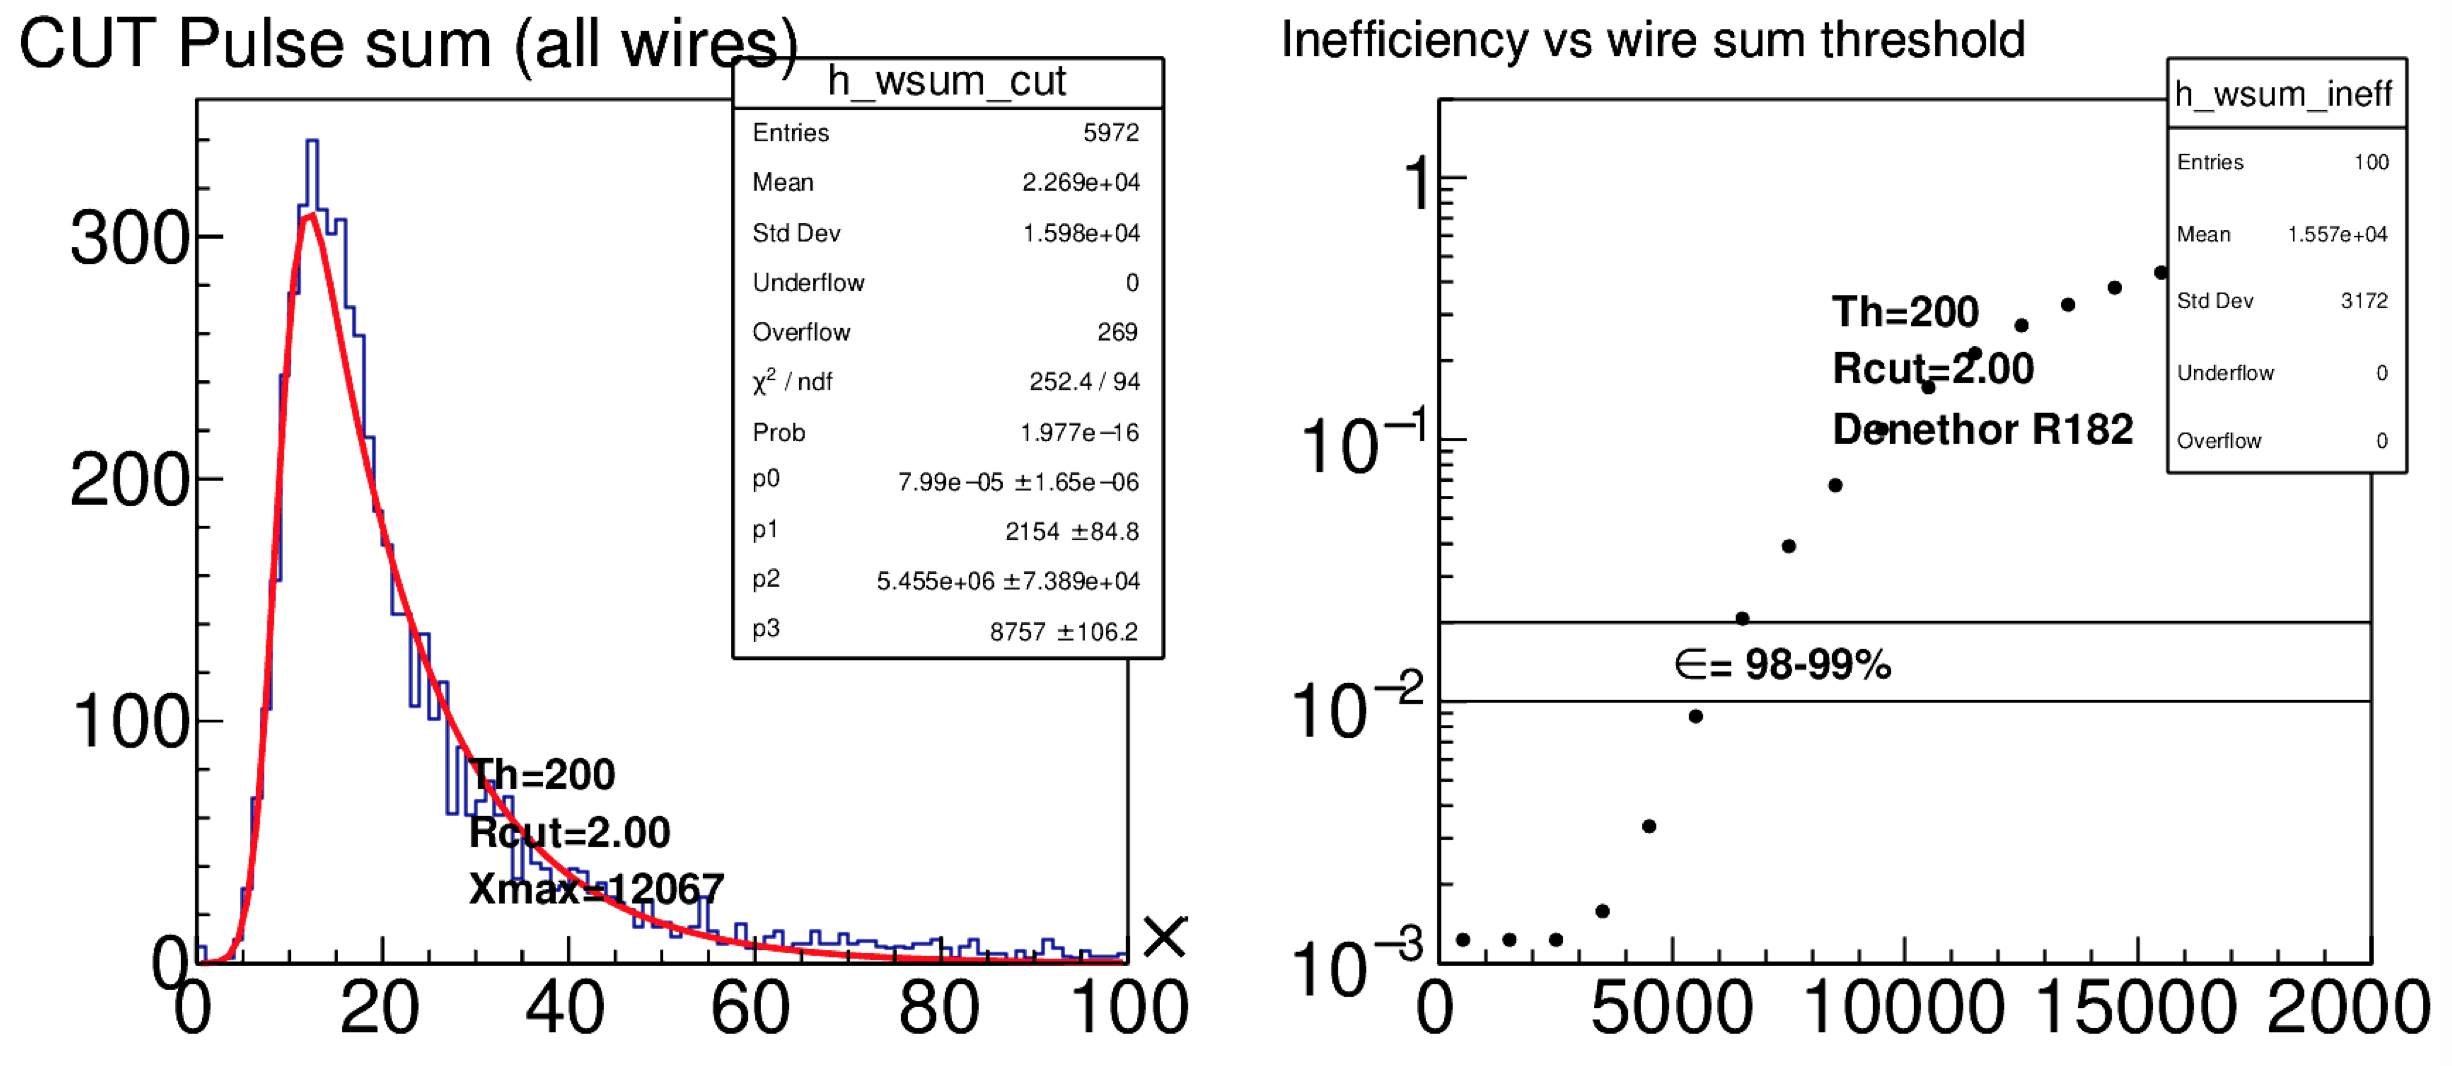
\includegraphics[height=5cm,clip=true]{Denethor_R182_HV1690_Th200_eff}
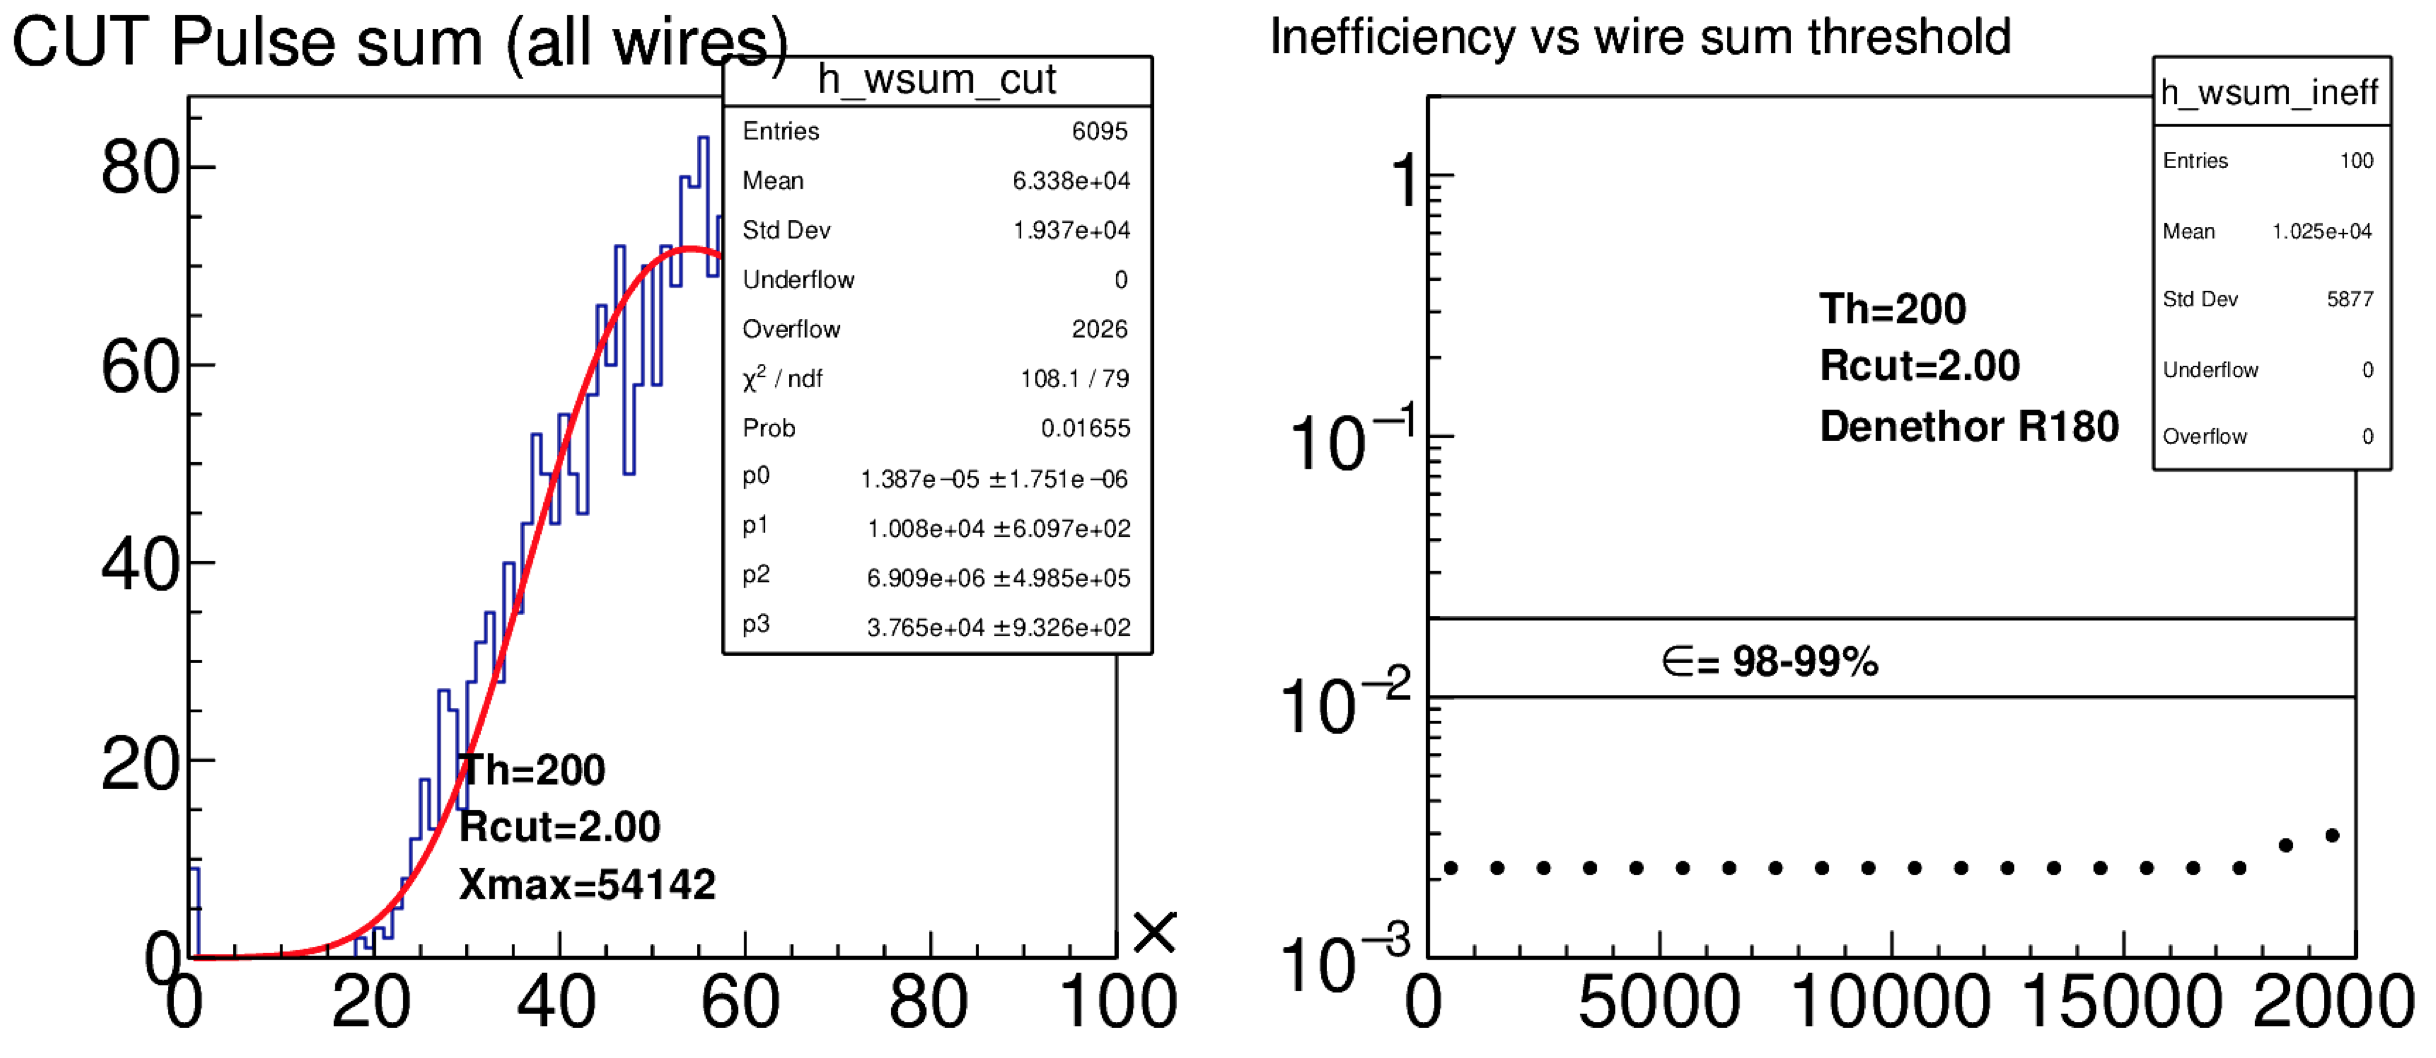
\includegraphics[height=5cm,clip=true]{Denethor_R180_HV1815_Th200_eff}
\caption{Top) Denethor HV=1690 V, Bottom) Denethor HV=1815 V. Left column) Sum of wire integrals. Right column) Inefficiency estimate vs threshold.
\label{fig:Denethor_HV1690_HV1815}}  
\end{center}
\end{figure} 

\begin{figure}[tbph]
\begin{center}
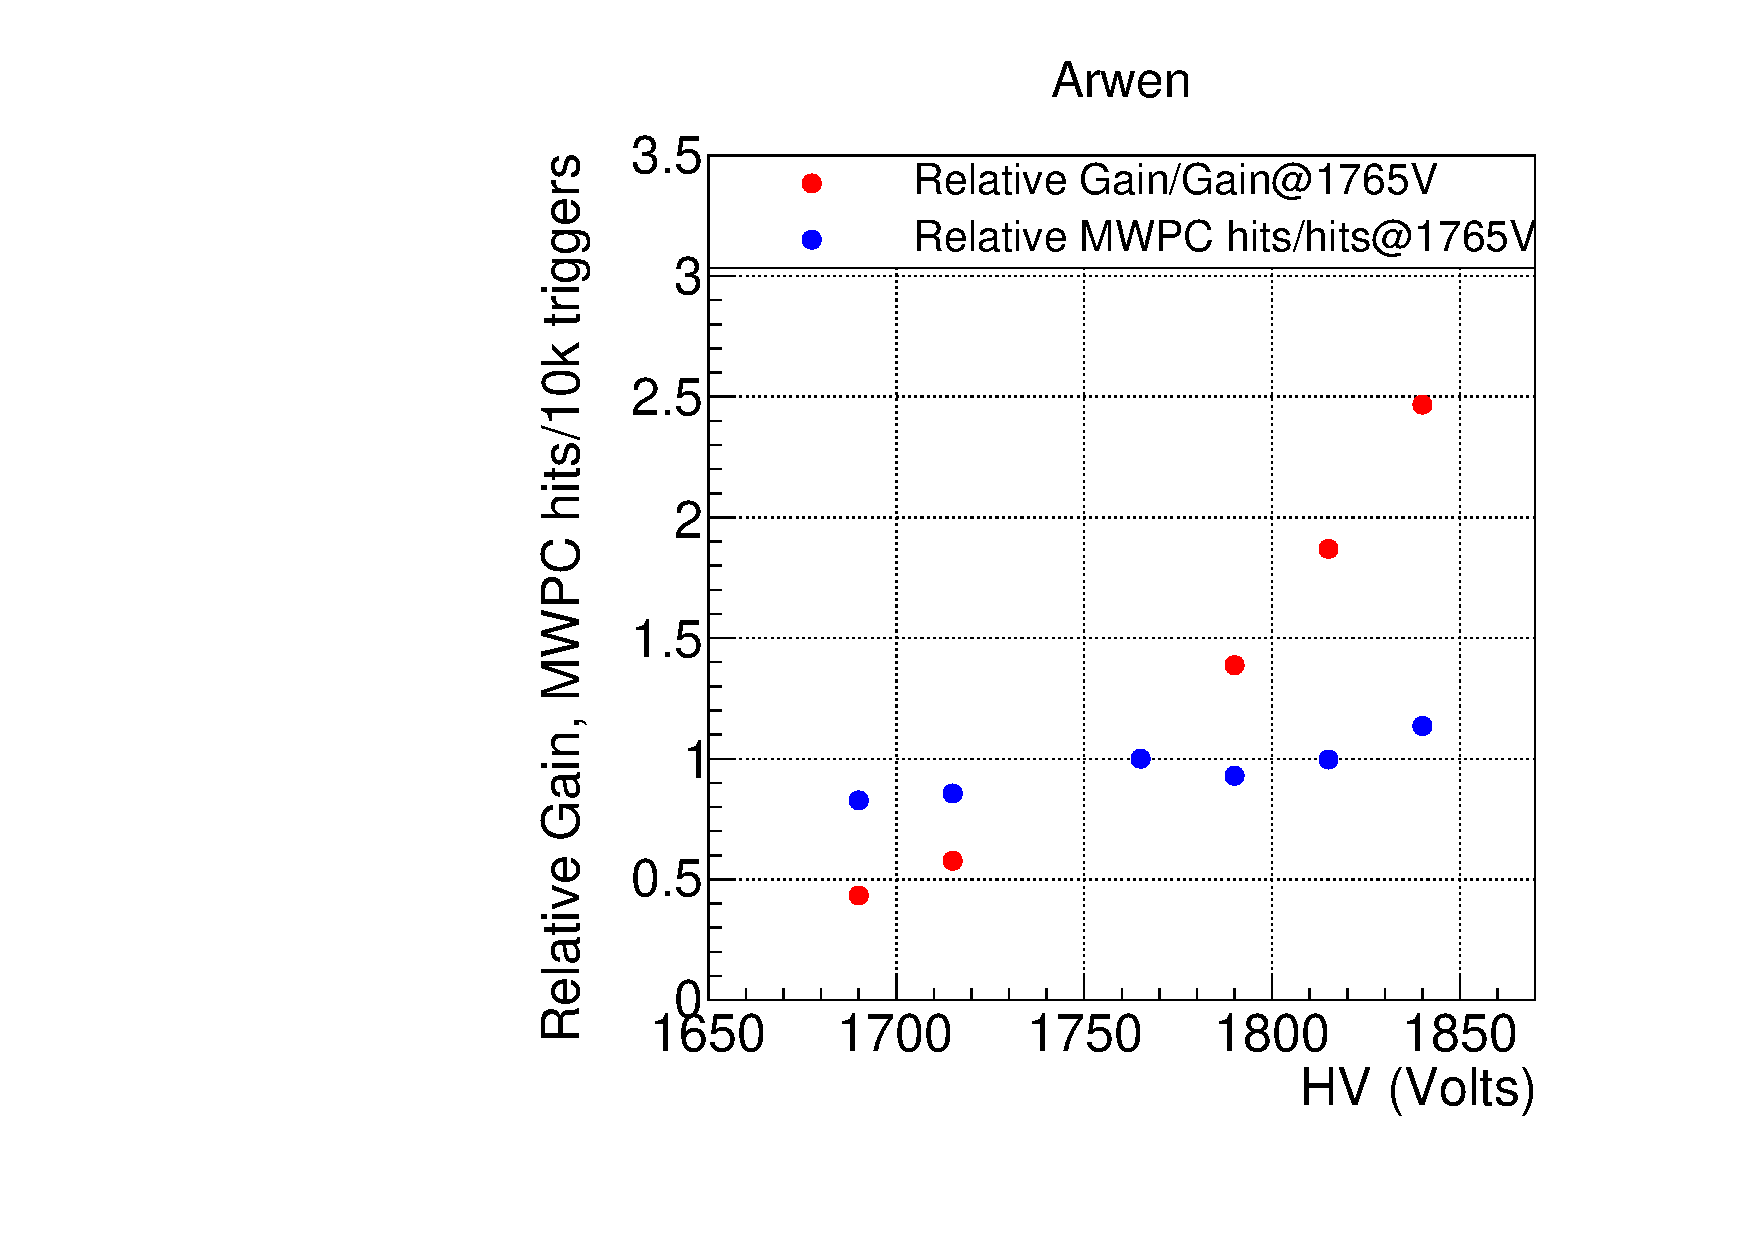
\includegraphics[height=7cm,clip=true]{plot_Arwen_HVscan}
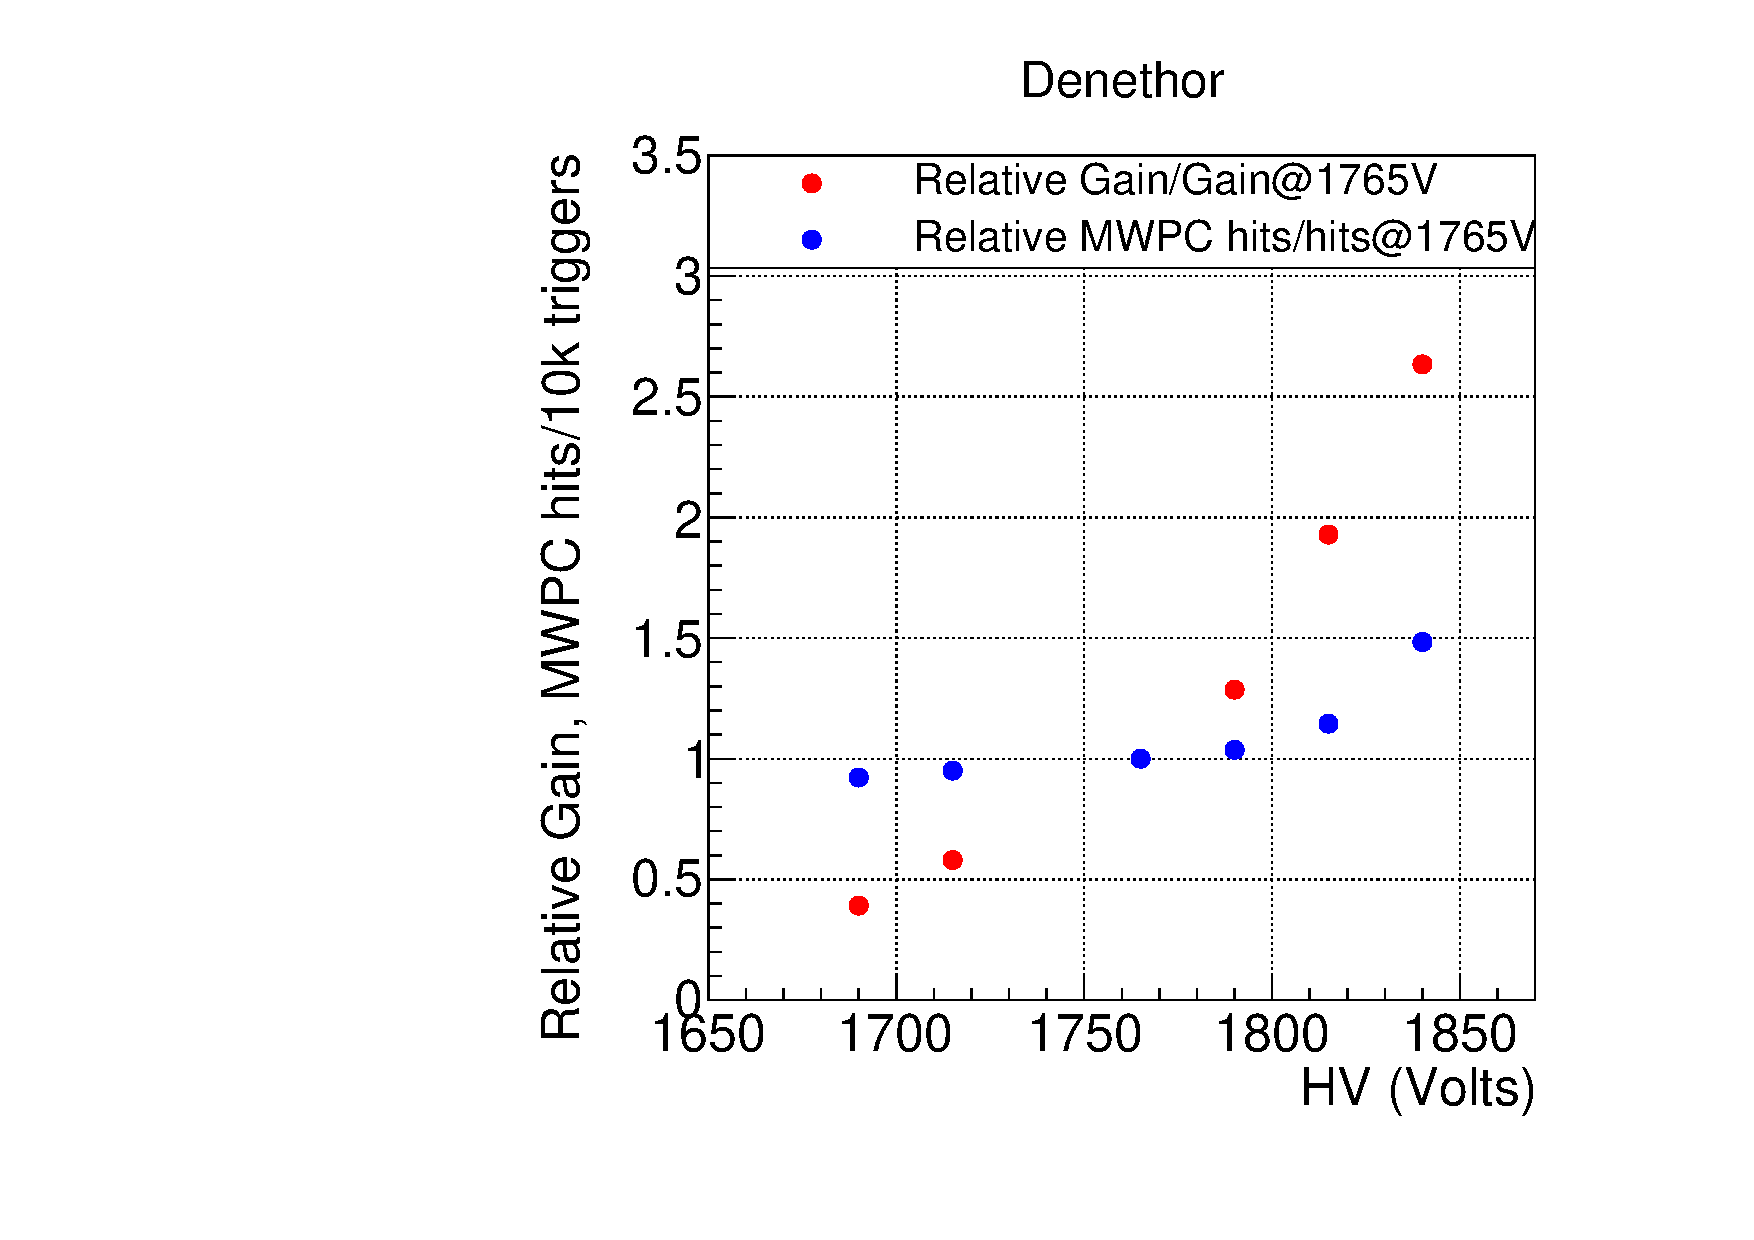
\includegraphics[height=7cm,clip=true]{plot_Denethor_HVscan}   
\caption{Rate and gain as a function of voltage for Left) Arwen and Right) Denethor.
\label{fig:plot_HVscan}}
\end{center}
\end{figure} 


\begin{figure}[tbph]
\begin{center}
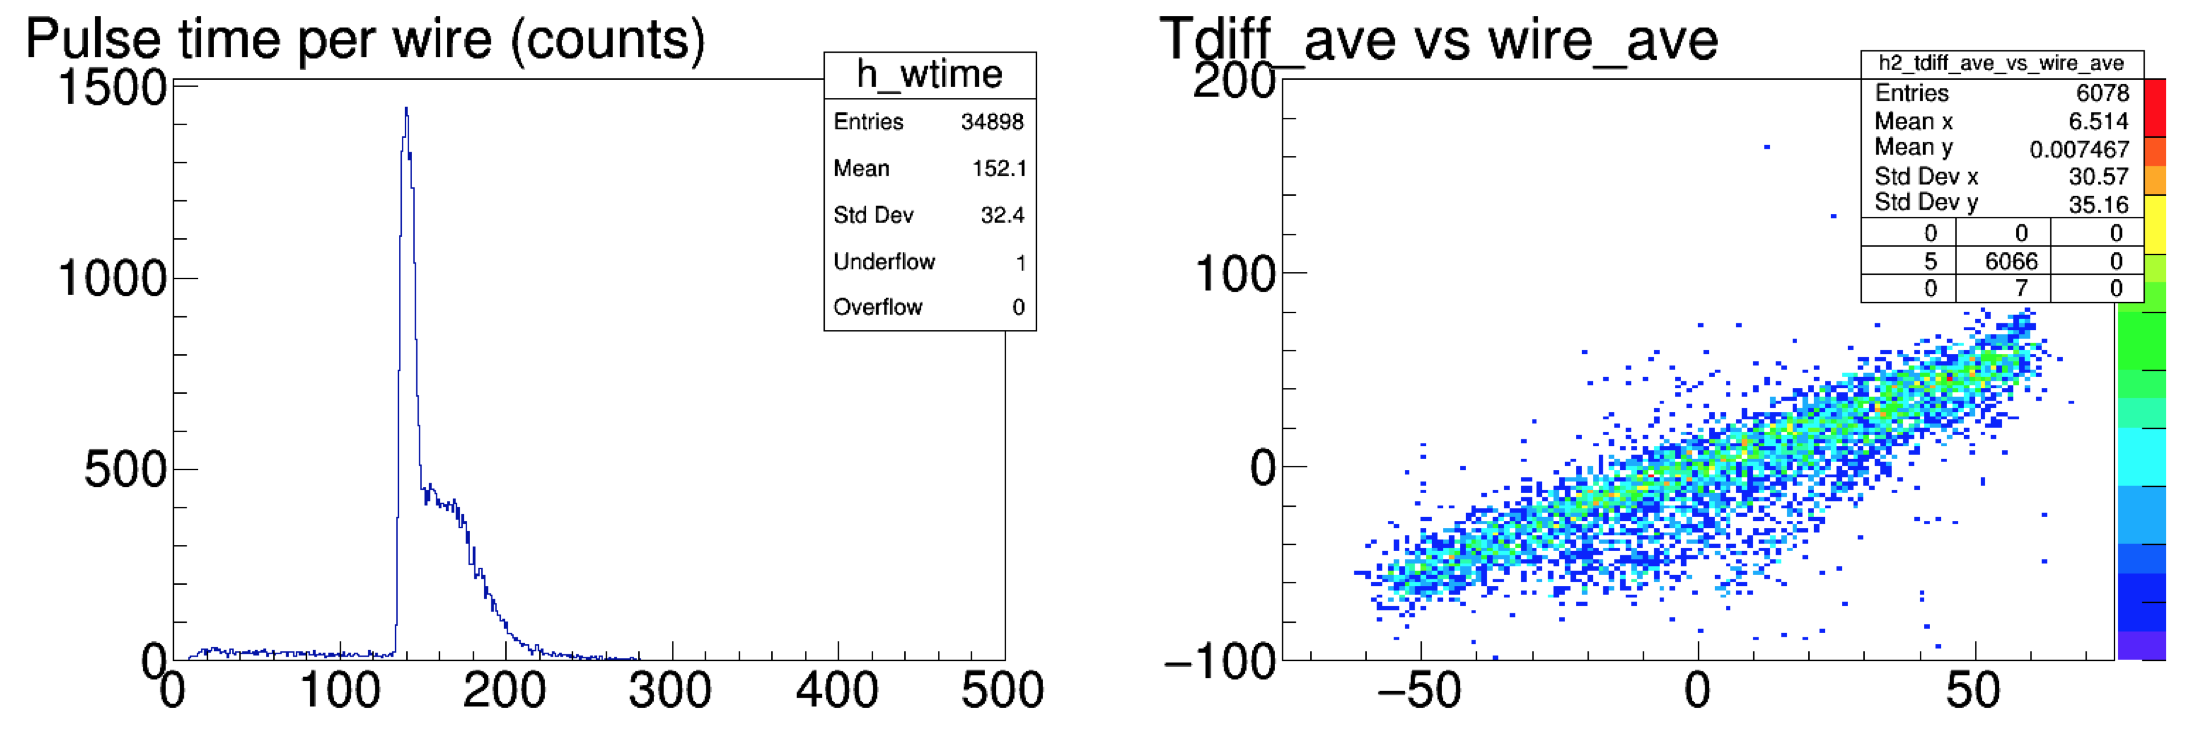
\includegraphics[height=5cm,clip=true]{Denethor_R183_HV1840_Th200}
\caption{Deterioration of validation plots for Denethor at HV=1840\,V. Left) Drift time distribution, Right) Correlation between scintillator positions and wire number.
\label{fig:Denethor_R183_HV1840_Th200}}
\end{center}
\end{figure} 

\section{Electronic noise  \label{sec:noise}}
Two of the chambers, Frodo and Galadriel, exhibit electronic noise that is recognizable as an oscillatory pattern on the measured baseline. Examples of waveforms can be seen in Fig.\,\ref{fig:Waveform_Galadriel_R157} where we show the baseline for wires with no signals as well as waveforms for wires with typical signals on top of the electronic noise. Note that the electronic noise is small compared to the minimum ionizing signal. Of course not all events show the electronic noise, as it appears random in time compared to the trigger. Various distributions of these chambers confirm the impact of the baseline noise on performance, as shown in Fig.\,\ref{fig:Galadriel_R157_Th000_hists}. These pathologic distributions can be compared to a quiet chamber (Arwen), illustrated in Figs.\,\ref{fig:MWPC_scint_correlation}, \ref{fig:Rint_to_peak} and \ref{fig:Arwen_R188_sum_nhits}. We note that the distribution of the sum of pulse integrals per event in Fig.\,\ref{fig:Galadriel_R157_Th000_hists} (bottom left) is actually quite clean (see also Fig.\,\ref{fig:efficiencies_e-f}). This is due to the fact that the electronic noise tends to average to zero in the integral. We note that it is possible to eliminate the electronic noise from these chambers by cutting all channels with pulses with peaks below 500-600 counts. This was done for the 
efficiency plots for Frodo and Galadriel in Section\,\ref{sec:eff}. 

Since we have six chambers that are very quiet, we do not believe that there is a problem with the design. Instead, it is likely due to improper grounding that is external to the chamber itself. Rory Miskimen has scheduled a trip to JLab to investigate the observed noise and finalize preparation of the chambers for the experiment.

\begin{figure}[tbph]
\begin{center}
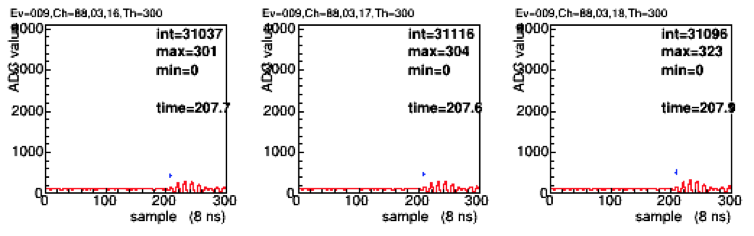
\includegraphics[height=4cm,clip=true]{Waveform_Galadriel_R157_Ev9}
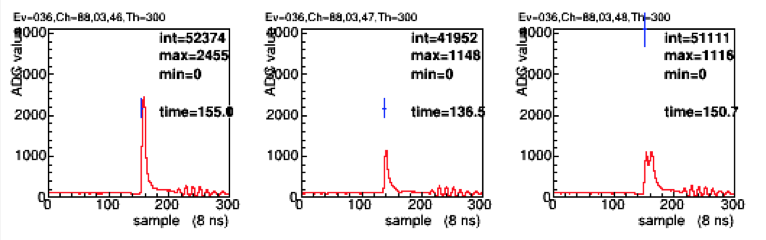
\includegraphics[height=4cm,clip=true]{Waveform_Galadriel_R157_Ev36}
\caption{MWPC Galadriel waveforms from R157. Note the oscillatory baseline indicative of electronic noise. The top row are waveforms from event 9 with no signal, and the bottom row are waveforms from event 36 with typical signals that are much higher than the noise level. The raw pulse integral and peak values are
also shown for each waveform. 
\label{fig:Waveform_Galadriel_R157}}
\end{center}
\end{figure} 


\begin{figure}[tbph]
\begin{center}
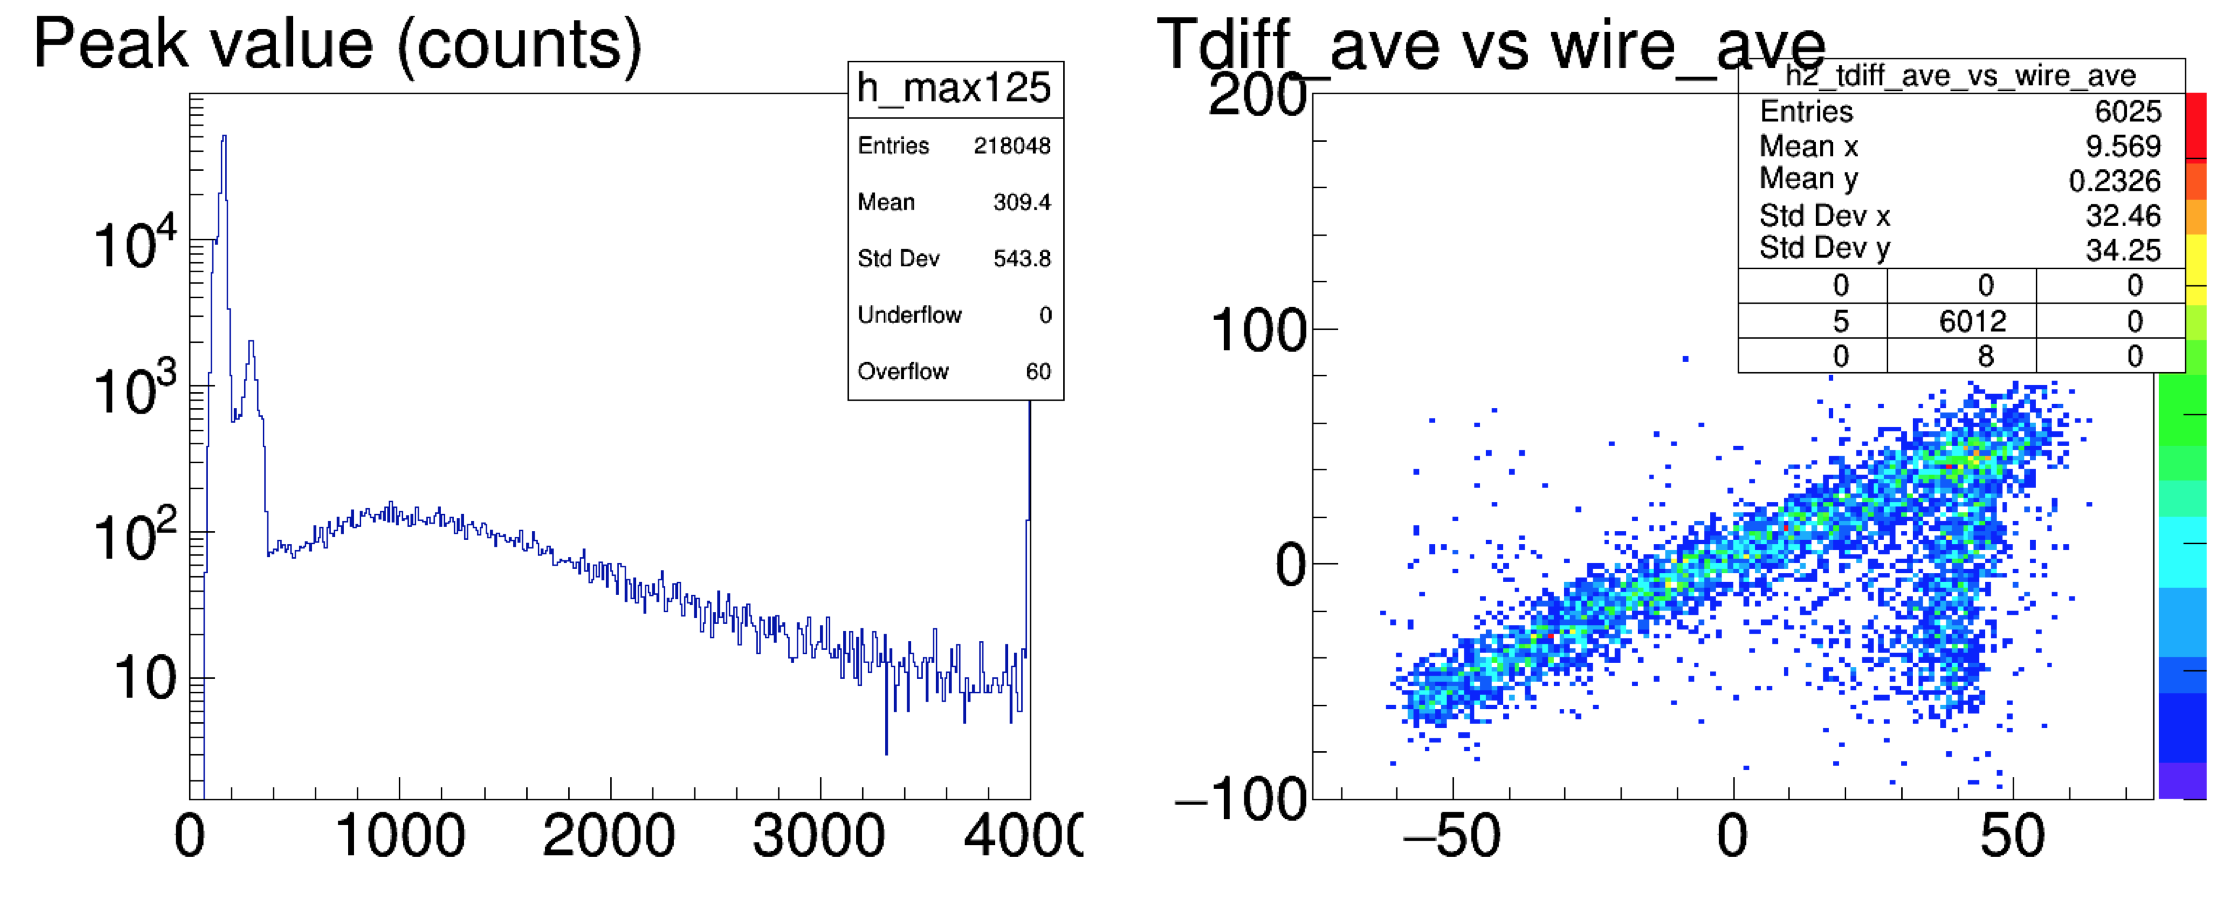
\includegraphics[height=6cm,clip=true]{Galadriel_R157_Th000_hists1}
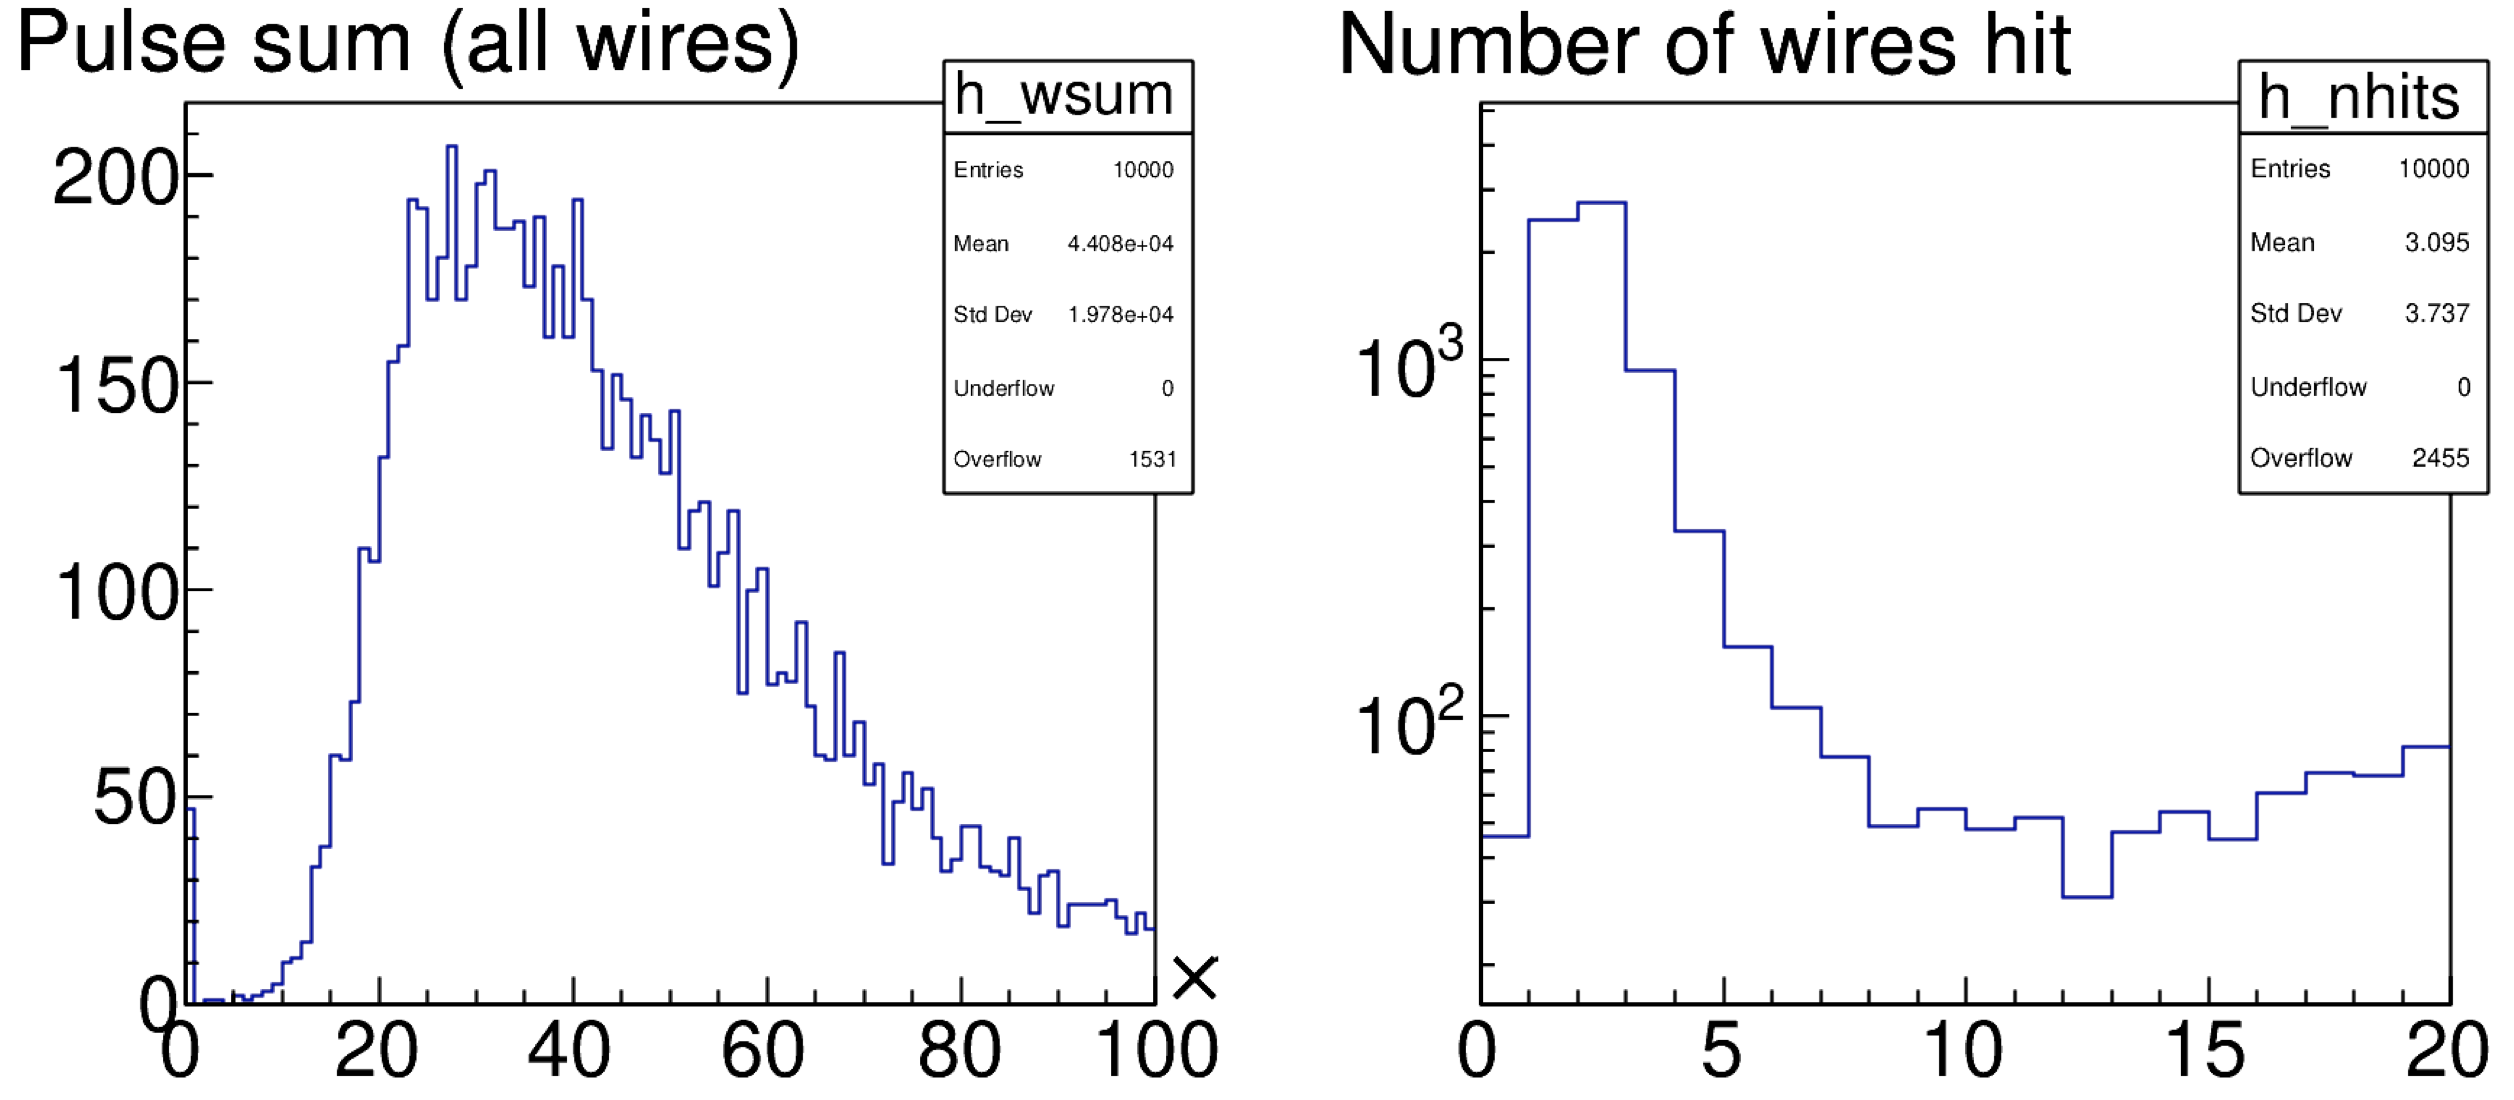
\includegraphics[height=6cm,clip=true]{Galadriel_R157_Th000_hists2}
\caption{Distributions for Galadriel illustrating the electronic noise. No explicit threshold cuts have been applied. Top left) Distribution of pulse peak values. Note the large quantities of pulses below about 500 counts, which are due to electronic noise. Top Right) Correlation between scintillator position and wire number. The vertical band is due to the electronic noise. The localization of this noise is artificial because the horizontal axis is the average wire number in the event. Bottom Left) The wire pulse sum is relatively clean despite the electronic noise, which it tends to average to zero in the integral. Bottom Right) The distribution of number of wires hit per event is often very large because the electronic noise affects whole regions of wires at once. 
\label{fig:Galadriel_R157_Th000_hists}}
\end{center}
\end{figure} 

\section{Conclusions} 
The Charged Pion Polarizability Experiment (CPP) requires a new muon detector, which will be located downstream of the Forward Calorimeter in Hall D. The muon detector requires six MWPC chambers. Eight chambers were fabricated at the University of Massachusetts and transported to JLab. We have tested the as-built MWPCs with cosmic rays in a test setup in the EEL building with a complete DAQ system that mimics the electronics to be used during the experiment. Six chambers were found to be very quiet with a measured efficiency of about 99.7\%, which satisfies the requirement for the experiment. The MWPCs operate reliably over a broad range of voltages. Two of the chambers have low levels of electrical noise. We anticipate that the source of the noise, likely incomplete grounding, will be identified and fixed. However, even in their present state  these chambers could serve as spares and used in the experiment by careful tuning of hardware thresholds.

%\nocite{*}
\bibliographystyle{unsrt}                                                                              
\bibliography{MWPC_production_testing}       

%\appendix
%\section{Derivation of method  \label{app:derivation}}
%\clearpage
%\newpage

\end{document}






